\documentclass{report}
\usepackage{amsfonts,amsthm,amsmath,latexsym}
\usepackage[margin=1.5in]{geometry}
\usepackage{complexity}
\usepackage{graphicx}
\usepackage[titles,subfigure]{tocloft}
\usepackage{scribe-book}

\usepackage{caption}
\usepackage{subcaption}
\usepackage{float}

\newcommand{\CYCLE}{{\sf CYCLE~}}
\newcommand{\FPSPACE}{{\sf FPSPACE~}}
\newcommand{\N}{{\mathbb{N}}}
\newcommand{\Z}{{\mathbb{Z}}}
\newcommand{\F}{{\mathbb{F}}}

%% For xy matrix
\input xy
\xyoption{all}
\CompileMatrices

\usepackage{tikz}
\usetikzlibrary{arrows}

\usetikzlibrary{calc,through,backgrounds,decorations.pathmorphing}

% Shows lecture titles and sections. Set 0 to list only chapters.
\setcounter{tocdepth}{1}

\begin{document}
\newpage
\setcounter{page}{1}
\pagenumbering{roman}  % Roman numbering in intro portion.
\begin{center}
{\bf \Huge Preface}         
\end{center}

\noindent
Matter to be entered here.

\newpage
\listofscribe          % For automatic scribe list generation.

\newpage
\tableofcontents

\setcounter{page}{1}
\pagenumbering{arabic}  % Arabic page numbering for lectures.

% Autogenerated using Makefile. DO NOT EDIT
\newpage \Lecture{Dinesh K.}{Jan 10, 2012}{4}{Quest for Structure in Counting Problems}
%\theme{Between $\P$ and $\PSPACE$.}
%\lectureplan{Counting problems and their structural complexity. Various attempts to develop the theory and the class $\#\P$. Basic containments.}

%We have seen several decision problems where we are interested in knowing the
%existence or non-existence of objects satisfying a certain property. An
%equally interesting question would be to ask the count of such objects. Such
%problems are called as counting problem.

In the previous lecture, we saw that the counting problem can be as hard as (or 
harder than) the decision problem as given an algorithm for counting problem
the decision problem reduces to just checking the count to be zero or not. We
also saw an easy decision problem \CYCLE whose counting version \#\CYCLE is
\NP-hard (by reduction from {\sf HAMCYCLE}) implying that easy decision
problems can also have corresponding counting problems hard. We also argued
that talking about counting problems still makes sense as the count value,
though exponential, can still be represented in polynomial number of
bits.

In this lecture, we will study counting problems and understand their
structural complexity. We shall also make attempts to develop the theory of
complexity classes capturing the counting problems (especially \#\P). We shall
also discuss their basic containments.

\section{Preliminaries}
Firstly, we fix our computation model where we have a Turing machine with an
input tape, work tape and an output tape. We are interested in the resources
used by the Turing machine - space (considering only the work tape) and time.

We want to capture the notion of counting formally. One such way is to see it
as computing a function $f : \Sigma^* \to \N$ where $\Sigma=\{0,1\}$ which
gives an integer value. So, how can we capture the notion of computing a
function? There are two possible ways of capturing function computation.
\begin{description}
\item[Variant 1] We say that a function $f$ is computable if each bit of the
output can be computed in some decision complexity class $\calC$.
\item[Variant 2] $f$ is computable if the value of the function computation
can be written down within the resource bounds.
\end{description}

Analogous to the decision problems, we define complexity classes for function
computation problems. A natural extension of \P~is \FP~ which is defined as
\begin{center}
\FP = $\{f \left | \right . f:\Sigma^* \to \N, f(x) \text{ for any } x \in
\Sigma^* \text{ can be written down in } poly(|x|) \text{ time}\}$
\end{center}

Now, we shall plugging in the two variants of function computation and see
which of them is more appropriate.

\section{Comparing the variants}
We quickly observe that the first and the second variant really coincides when we are talking
about deterministic computations. Let us do this analysis by attempting the definition of $\FP$.
Following the first variant $f \in \FP$ iff there exists an algorithm that can
compute each bit of $f$ in class \P. But since the algorithm is deterministic, this is  
equivalent to saying that $\forall~i$, the language defined by the $i^{th}$ bit 
$$L_{f_i} = \{ x : (f(x))_i = 1 \} \in \P$$
On the other hand, if each bit can be computed in polynomial time 
and since the count value can be represented in polynomial number of bits, for
evaluation, we just run a polynomial time algorithm polynomial times
which is still a polynomial. Hence we have an algorithm that satisfies the 
second variant.

Hence for deterministic polynomial time computation both variants are equivalent.
We can define other classes for deterministic computation 
like {\sf FL}(log space bounded function computation), \FPSPACE(polynomial
space bounded function computation). Containments of these classes are
analogous to their decision versions. We leave the proof as an exercise.

\begin{lemma}
${\sf FL} \subseteq \FP \subseteq \FPSPACE$
\end{lemma}

Now we turn into the non-deterministic world. 
Following variant 1 of definition of function computation, we must have each
bit computable in class \NP. But variant 2 is not useful because an non-deterministic 
poly time Turing machine by our model is not set to output a value. How can we
capture the function computation for a non-deterministic machine for decision
problems which works by guess-verify mechanism?

Now, consider the non-deterministic algorithm
we had for \SAT, which does guessing of an assignment and verifying it. 
We can observe the following additional property.
\begin{observation}
Number of satisfying assignments is exactly equal to the number of accepting
paths.
\end{observation}
This leads to the question as to whether this is accidental or is there some
hidden structure? It also assigns a function value to the non-deterministic Turing machine.
This motivates us to give a new model, for us to call $f$ is computable by a non-deterministic polynomial time Turing machine.

\begin{definition}
$f$ is $\#\P$ if there exists a non-deterministic Turing machine $M$ running in time $p(n)$ such that 
$\forall x \in \Sigma^*$, $f(x) = \left| \{ y \in \{0,1\}^{p(n)}  : M \textrm{ accepts on path $y$ } \} \right|$.
\end{definition}

\begin{remark}
The RHS is also the number of accepting paths of $M$ on $x$ if the lengths of all paths are equal to $p(n)$.
We remark that this can be achieved without loss of generality. That is, from an arbitrary TM $M$, we can get to a new TM $M'$ which has the same number of accepting paths, such that the number of accepting paths on any input $x$ remains the same. We recall our observation that for length of all non-deterministic paths of an \NP~machine on any input can be made equal without changing the accepted language\footnote{In particular, we showed that a language $A \in \NP$ if and only if there is a language $B \in \P$ and a polynomial $p(n)$ such that $x \in A \iff \exists y \in \{0,1\}^{p(n)} : (x,y) \in B$} . But this construction makes the language accepted the same, and need not keep the number of accepting paths the same. We modify it slightly to achieve our goal.  Indeed, if a path is shorter than $p(n)$ bits and decided A/R, we extend it to the required length using a binary tree of paths rooted at that node and make the left most path (in this binary tree) report A/R respectively and make all other paths reject. The number of accepting paths does not change due to this construction.
\end{remark}

\begin{remark}
Try this as an exercise. Initiate the thought process on : how does this definition compare with variant 1? What does computing/testing each bit to be 0/1 mean?
\end{remark}

%\begin{proof}
%Recall that, 
%\begin{center}
%$ \calL \in \NP \iff \exists \calB \in \P \text{ and a polynomial } p(n)
%\text{ such that} $ 
%$(x \in \calL \iff \exists y \in \{0,1\}^{p(n)}, (x, y) \in \calB )$
%\end{center}
%Hence  a non-deterministic machine $N$ for $\calL$ just need to guess $p(n)$
%bits and run the verifier to validate the guess. Hence every non-deterministic
%path will be of length $p(n)$.
%\end{proof}
%Hence our observation actually follows from the definition. This gives us a
%better characterisation.

%\begin{definition}
%$f$ is computable by a non-deterministic Turing machine $M$ running in 
%ime $p(n)$ if $ \forall x \in \Sigma^*, f(x) = |\{ y \in \{0,1\}^{p(n)} | 
% \text{ accepts on path } y \}|$. The class of functions for which such 
%non-deterministic Turing machines exists is called \#\P (``sharp P")
%\end{definition}

Counting version of \SAT~denoted as \#\SAT~can be defined as 
\[ \#\SAT(\phi) = |\{ \sigma | \phi(\sigma) = 1, \sigma \text{ is a boolean
assignment to variables in } \phi \}| \]
It follows from our observation that $\#\SAT \in \#\P$, since we can give a
non-deterministic machine (i,e. a machine for \SAT) where number of accepting
paths equals to the number of satisfying truth assignments. It can also be
shown that $\#\CYCLE \in \#\P$.

\begin{claim}
$\#\CYCLE \in \#\P$
\end{claim}
\begin{proof}
Following is a non-deterministic Turing machine $N$, such that number of
cycles equals number of accepting paths.

$N$ = `` On input $G$,
\begin{enumerate}
\item Guess subsets $V' \subseteq V(G)$ and $E' \subseteq E(G)$ 
non-deterministically.
\item Accept iff $V', E'$ form a simple cycle. "
\end{enumerate}

Now it follows that $\#\CYCLE(G) = |\{ \# \text{ of accepting paths of } N
\text{ on } G \}|$ since any cycle can uniquely be characterised by an edge set
and a vertex set.
\end{proof}

\section{Basic Containments}
In the functional world, we have the following scenario.
\begin{center}
\FPSPACE \\
$\vert$ \\
\FP \\
$\vert$ \\
{\sf FL }
\end{center}

So where does set of functions, $\#\P$ lie? We will argue that $\#\P$ lies between 
\FP and \FPSPACE thus replicating the picture in the decision world.
\begin{lemma}
$\#\P \subseteq \FPSPACE$
\end{lemma}
\begin{proof}
Given a non-deterministic poly time Turing machine $M$ computing function $f$,
we just need to do a simulation in deterministic poly space. This can be done by
simulating $M$ over all non deterministic paths while reusing space across the
paths. Since length of any path is polynomially bounded, space used will also
be polynomial. In the process we need to keep the count of accepting paths
which can be $\le 2^{p(n)}$ but still representable with $p(n)$ bits in
binary. Hence space requirement is only polynomial in input length.
\end{proof}

\begin{lemma}
$\FP \subseteq \#\P$
\end{lemma}
\begin{proof}
Given an $\calL \in \FP$, there exists a deterministic Turing machine $M$ which
$\forall x \in \calL$ writes $f(x)$ in $p(n)$ time where $p$ is a polynomial
and $n = |x|$. To show that $\calL \in \#\P$, we need to construct a
non-deterministic  such that
\begin{center}
No of accepting paths = $f(x)$.
\end{center}
$N$ can compute $f(x)$ by simulating $M$. Let the value obtained be $k$. Now,
$N$ must have exactly $k$ accepting paths. This can be ensured by guessing
$\lceil \log k \rceil$ bits and accepting all the paths whose address have
binary representations  $\le k$ and rejecting the remaining paths.

$N$ runs in poly time since $f(x)$ computation (simulation of $M$) takes only
polynomial time. Even though $f(x)$ is exponential, number of bits guessed is
$\lceil \log f(x) \rceil$ which will be polynomial in $n$. Hence depth is
polynomially bounded. Also number of accepting paths equals $f(x)$ by
construction. Thus $N'$ is a \#\P machine accepting $\calL$. Hence $\calL =
L(N') \in \#\P$.
\end{proof}

\begin{figure}[htp!]
\centering
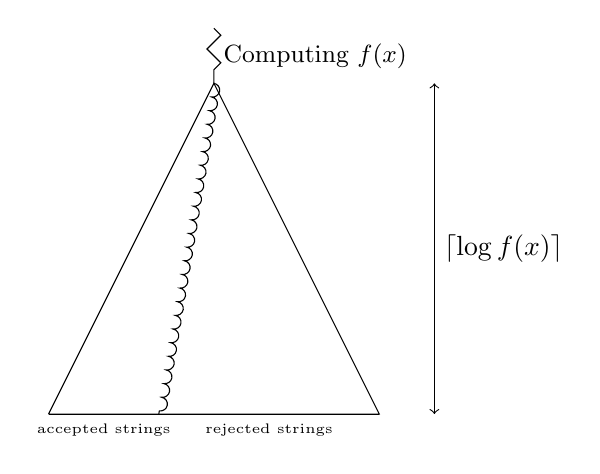
\begin{tikzpicture}[scale=0.7]
\coordinate (T) at (3,7);
\coordinate (A) at (0,0);
\coordinate (B) at (6,0);
\coordinate (C) at (3,6);
\coordinate (M) at (2,0);
\draw [decorate,decoration=zigzag] (T) -> (C) node[midway,right]
{ {\small Computing $f(x)$ }};
\draw (A) -- (M) node[midway,below] { {\tiny accepted strings}} ;
\draw (M) -- (B) node[midway,below] { {\tiny rejected strings}} ;
\draw (A) -- (B) -- (C) -- (A);
\draw [decorate,decoration=bumps] (C) -> (M);
\draw [<->] (7,0) -- (7,6) node[midway,right] {$\lceil \log f(x) \rceil$};
\end{tikzpicture}
\end{figure}

It can be observed that if function computation can be done in polynomial time
then $\P = \NP$. This is because solving decision problem amounts to checking
if the corresponding counting function gives a non zero value or not hence
making decision problem easy if function computation is in \P. 
\begin{lemma}
$\#\P = \FP \implies \P = \NP$
\end{lemma}

An interesting question would be to ask if the converse it true? That is 
\begin{center}
Does $\P = \NP \text{ imply }  \#\P = \FP ?$
\end{center}
We will address this and show a weaker implication (that is, based on slightly stronger LHS) in the next lecture.


\newpage \Lecture{Prasun Kumar}{Jan 12, 2012}{5}{$\FP$ vs $\#\P$ question}
%\theme{ Between $\P$ and $\PSPACE$.}
%\lectureplan{ $\FP$ vs $\#\P$ question, a counter part in the decision world. The class PP. PP vs P is equivalent to FP vs $\#\P$.}

We know $(\#\P = \FP) \implies (\P = \NP)$. In the last lecture we left the question about the converse.
i.e., is it true that, $(\P = \NP) \implies (\#\P = \FP)$?

In this lecture, we will show a weaker version of the above containment.
We will define a new class of languages $\PP$ (probabilistic polynomial time)
in decision world, that contains $\NP$, and will show that if we make a stronger assumption $\PP = \P$ (seemingly stronger than $\NP = \P$) we get the required implication.  We will show in particular that $\PP = \P \iff \#\P = \FP$.

\section{Complexity Class \PP}
For exploring the complexity class, we revisit the definition of $\NP$.
With respect to a "branching" Turing machine(NTM) (which can branch at each computation by using a guess bit), we have two different classes of languages as follows, which differs in their acceptance conditions. We denote for a machine $M$, by $\#acc_M(x)$ as the number of accepting paths. Let the machine run for $p(n)$ time on each path.
\begin{itemize}
\item $\NP$ = $\{$L : $\exists$ branching TM $M_1$, x $\in$ L $\iff \#acc_{M_1}(x) \ge 1 \}$.
\item $\coNP$ = $\{$L : $\exists$ branching TM $M_2$, x $\in$ L $\iff \#acc_{M_2}(x) \ge 2^{p(n)} \}$.
\end{itemize}

In terms of number of accepting paths on input $x$, the above classes
represent the extremes.  On one side, in $\NP$ we talk of atleast one
accepting path, and on the other side, in $\coNP$ we talk of all
accepting paths. To understand the structure of these classes we can
ask the variant of this as : what different class of languages do we
get if we set the accepting condition as the number of accepting paths
being more than a fraction of the total number of paths on input {\em
  x}. A simpler situation is to consider the fraction to be half and the
corresponding class of languages is called \PP (probabilistic
polynomial) which is defined as follows. We will come across other variants in
the later lectures.

\begin{definition}
$\PP$ =$\{$L : $\exists$ NTM $M$, x $\in$ L $\iff \#acc_{M_1}(x) > 2^{p(n)-1} \}$
\end{definition}

We first understand this complexity class with respect to the other ones we have already seen. We start with the following proposition.

\begin{proposition}
\label{prop}
$\NP \subseteq \PP$.
\end{proposition}
\begin{proof}
Let $L \in \NP$  via a nondeterministic turing machine $M$,  $ x \in L \iff M$ has atleast one accepting path on $x$. 
Our aim is to give another turing machine $M'$ for the same language $L$ such that
$x \in L \iff M'$ has more than half of the total number of paths as accepting paths on $x$.\\
Description of $M'$ (on input $x$):
\begin{enumerate}
\item Simulate $M$ on $x$.
\item If $M$ accepts then choose one bit nondeterministically and accept in both branches.
\item If $M$ rejects then choose one bit nondeterministically,accept in one branch and reject in other.
\end{enumerate}

As we remarked in the last lecture, we can assume without loss of generality that the height of computation tree of $M$ on $x$ is exactly $p(n)$ for some polynomial $p$. Since the total number of paths for $M'$ on input $x$ is $2^{p(n)+1}$, it suffices to prove that $x \in L \iff \#acc_M(x) > 2^{p(n)}$.
Let $x \in L$. Since $M$ has at least one accepting path on $x$. Since $M'$, by construction, creates an imbalance (in count) between the number of accepting and rejecting paths precisely when $M$ accepts,  the number of accepting paths in $M'$ will be more than the number of rejecting paths. Thus $\#acc_M(x) > 2^{p(n)}$. \\
If  $x \not\in L$, all paths reject in $M$ on input $x$, and thus  number of accepting and rejecting
paths in $M'$ on input $x$ are exactly equal and each of themsame is equal to $2^{p(n)}$.
\end{proof}

A similar proof will also show that $\coNP$ is contained in
$\PP$. Thus we have the following containment relationship among
different classes of languages
 
\begin{center}
\PSPACE \\ 
$\vert$ \\
\PP \\
$\vert$ \\
\NP \\
$\vert$ \\
\P
\end{center}

Now we will prove the main theorem of the lecture which characterizes the $\FP$ vs $\#\P$ question in the decision world.

\begin{theorem}
 $(\#\P = \FP) \iff (\PP = \P)$
\end{theorem}
\begin{proof}
($\Rightarrow$) Assume $\#\P = \FP$, our aim is to prove $\PP = \P$. The reverse containment follows since we know $\NP \subseteq \PP$ by proposition\ref{prop}. Now we show that $\PP \subseteq \P$ . Let $L \in \PP$
via a machine $M$ running in time $p(n)$ for some polynomial $p$, such that $x \in L \iff \#acc_M(x) > 2^{p(n)-1}$.
Define the function, $f(x) = \#acc_M(x)$. By definition $f \in \#\P$ and hence $f \in \FP$. There is a deterministic polynomial time Turing machine $N$ which on input $x$ outputs the value of $f(x)$. Given an $x$, to test whether it is in $L$ or not, it suffices to test whether whether the MSB of the binary representation of $f(x)$ is 1 or not. This can be done by simply running the machine $N$ on $x$ and testing the MSB of the output. Hence $L \in P$.

($\Leftarrow$) Assume $\PP = \P$, our aim is to prove $\#\P = \FP$. The reverse direction is easy. $\FP \subseteq \#\P$ as we argued in the last lecture. To show the forward direction, let $f\in \#\P$ via $M$ such that $\forall x \in \Sigma^*$, $f(x)=\# accept_M(x)$. Note that the naive approach to compute $f(x)$ is to compute the number of accepting paths in computation tree of height $p(n)$ will take exponential time. But it suffices to find the minimum $0 \le k \le 2^{p(n)}$ such that :
\begin{equation}
\label{eqn}
k+\#acc_M(x) > 2^{p(n)}
\end{equation}
Indeed, the minimum is achieved when $k = k_{min} = 2^{p(n)} - \#acc_M(x) + 1$. Thus $\#acc_M(x) = 2^{p(n)} - k_{min} +1$. This is an indirect way of finding out $\#acc_M(x)$ and we are moving towards using our assumption that $\PP = \P$.

We have  search problem in hand; to search for the minimum $k$($k_{min}$) satisfying equation (\ref{eqn}). We do this by binary search over the range $0 \le k \le 2^{p(n)}$. We solve the decision problem first. {\sf Given $x$ and $k$, check if $k+\#acc_M(x) > 2^{p(n)}$}.

For this, we construct an another Turing machine $N$ such that the number of accepting paths is exactly $k+\#acc_M(x)$ and the total number of paths is $2^{p(n)+1}$. Assume such a construction exists. Define a language $A \subset \Sigma^*$ such that $x \in A \iff k+\#acc_M(x) > 2^{p(n)}$. Thus $x \in A \iff \#acc_N(x) > 2^{p(n)}$. This implies that $A \in PP$ (via the machine $N$ !) and hence $A \in P$ by assumption. Given $x \in \Sigma^*$ we can test if $k+\#acc_M(x) > 2^{p(n)}$ by testing if $x \in A$ or not, which can be done in polynomial time. Now we can do this construction and simulation through a binary search in order to find the minimum value of $k$ that satisfies our inequality.

To complete the proof, we give the construction of $N$ (for a given $k$). 
We first construct a machine $M_k$ that runs in time $p(n)$ and has exactly $k$ accepting paths. 
We slightly modify the idea in the previous lecture to do this. Let $\ell = \lceil \log k \rceil$.
The machine $M_k$ guesses a $y \in \{0,1\}^{p(n)}$ and {\em accepts} if the first $\ell$ bits of $y$ in binary represents a number less than $k$ and the last $p(n)-\ell$  bits is all-zero (lexicographically first path) and {\em reject} otherwise.

We combine $M_k$ and $N$ (both using exactly $p(n)$ non-deterministic bits), to get the machine $N$. The machine $N$ on input $x$ guesses $1$ bit and on the $0$-branch it simulates $M_k$ on $x$ and on the $1$-branch it simulates $M$ on $x$. Clearly $\#acc_N(x) = \#acc_{M_k}(x) + \#acc_{M}(x) = k+\#acc_{M}(x)$. The length of each path is exactly $p(n)+1$ and hence total number of paths is $2^{p(n)+1}$.
\end{proof}




\newpage \Lecture{Sunil K S.}{Jan 13, 2012}{6}{$\#\P$-Completeness}
%\theme{Between $\P$ and $\PSPACE$.}
%\lectureplan{Structure of Reduction in Counting world}

Thus we motivated to answer the questions. We saw $(\#\P=\FP) \iff (\P=\PP)$ in decision world. 
This motivates understanding structure in the counting world.
We start with the notion of reductions. 

\section{Reduction in Counting World}

Our aim is to come up with a notion of $\#\P$-completeness and show structural classification of counting problems. Informally, we have seen counting problems that are hard to solve. We want our notion of hardness to capture this as closely as possible. We consider some natural options for such a definition and proceed from there.

\begin{description}
\item{\textbf{Attempt 1:}}
	Let A,B be two languages. In decision world $A \leq ^p_m B$ if and only if
	\begin{enumerate}
		\item $x\in A\Longleftrightarrow \sigma\in B$.
		\item $\sigma : \Sigma ^*\rightarrow\Sigma^*$ is polynomial time computable.
	\end{enumerate}
	Translating the above statements into counting scenario.
	\begin{enumerate}
		\item $\sigma$ is polynomial time computable.
		\item $f(x)=g(\sigma(x))$.
	\end{enumerate}
	Two lectures back we showed $\SAT$ can be decided if $\#CYCLE$ can be computed. But following the above attempted notion of a reduction, we get the following.
\begin{equation}
\label{eqn:parsi}
	\#\SAT(\phi)=\#CYCLE(\sigma(\phi))
\end{equation}
	
	But if such a reduction exists, then we can solve $SAT$ by checking if $\#SAT(\phi)=\#CYCLE(\sigma(\phi))$, which in turn can be done in polynomial time. Thus, if we impose this strictness then in $\#\P$ only counting versions of $\NP$-complete problems will be hard. Notice that the issue here is that the reduction is set to preserve the number of certificates !. %The reductions which has this property are called {\em parsimonious} reductions.
	
	Let us make some preliminary observations. What if we allow factors in equation\ref{eqn:parsi}? Could this save us? No, still if such a reduction exists, we can decide $\SAT$  by counting the value of $\#CYCLE$. Indeed, there would not have been a problem if there was a "+1" on the right hand side of the above expression, such that the zeroness of $\#\SAT$ does not carry over to the zeroness of $\#CYCLE(\sigma(\phi))$. This shows that may be we should allow non-trivial computations after the query to the function $\#CYCLE$. Since we would also like structural composibility and transitivity of reductions, this naturally leads to the attempt 2, in its generality.
	
\item{\textbf{Attempt 2:}}
We attempt now a generalization of the notion of Turing reductions.
\begin{definition} 
	We say that a function $f \leq g$ if $f\in FP^g$. That is, if there exists a functional oracle Turing machine\footnote{A functional oracle TM is similar to the normal oracle Turing machine, but since the output of the oracle query is not a 1-bit, instead of $q_{yes}/q_{no}$ as the two states to which the machine moves after the oracle answers, the machine has has an oracle output tape for the oracle to write the function value.} 
with queries to $g:\Sigma^*\rightarrow$ $\mathbb{N}$ that given any $x\in \Sigma^*$ can compute $f(x)$. 
	\\A function $g$ is $\#\P$-hard if $\forall f\in \#\P, f\leq_m^p g$. $g$ is complete for $\#\P$ if $g \in \#\P$ and $g$ is $\#\P$-hard.
\end{definition}
\end{description}

\begin{theorem}
 $\#\SAT$ is $\#\P$-complete.
\end{theorem}
	\begin{enumerate}
		\item $\#\SAT \in \#\P$: $\exists$ a non-deterministic turing machine polynomial time which guesses assignments (bit by bit), verifies the same, accepts if it satisfies the formula, and rejects otherwise. No assignment is guessed by two different non-deterministic computation paths. Hence the number of accepting paths will precisely be equal.
		\item $\forall f \in \#\P, f \leq_m^p \#\SAT$: Let $f\in \#\P$ via a machine $M$ such that $\forall x \in \Sigma^*, f(x)=\#acc_M(x)$.
	\begin{description}
	\item \textbf{Cook-Levin Theorem - Revisited.}
	\begin{center}
	$L\in \NP \Longrightarrow L\leq^p_m \SAT$.
	\end{center}
	Let $L\in \NP$, via machine $M$ such that $x\in L \Longrightarrow M$ has an accepting path.
	We construct $\phi_{(M,x)}$ from computation history such that 	$ M$  has an accepting path implies $ \phi_{(M,x)}$ is satisfiable. For every accepting path, we have a satisfying assignment and for every satisfying assignment there is a corresponding accepting path too. Moreover, this map is There is a one-to one mapping between the set of accepting paths and the set of satisfying assignments. The certificates corresponds to the first set is the choice of non-deterministic bits and for the second set is the satisfying assignments. Such reductions are called \emph{Parsimonious reductions}. An additional point is that this certificate bijection is polynomial time computable. That is given an accepting path of the machine $M$ the reduction also gives you a way to transform it into a satisfying assignment of the formula and vice versa. Reductions satisfying the latter property are called {\em Levin reductions}. Note that, in order to prove $\NP$-completeness, the reduction neither need to be parsimonious nor it should be Levin reduction. It is an additional structural property that the reductions seems to satisfy. Interestingly, the $\NP$-complete reductions that we have seen in the last course (like the SAT to 3SAT, 3SAT to independent set, Independent set to Vertex Cover), has this additional structural property. Thus all of them are $\#\P$-complete by our definition.
\end{description}
\end{enumerate}

We have already talked out one example of a decision problem which is in $\P$, but the counting version seems to be as hard as $\NP$. We will consider another similar problem  and show that the counting version can be shown to be $\#\P$-complete as well. Indeed $\#CYCLE$ is also $\#\P$-complete. We introduce the problem now:

\section{Perfect Matching in a graph}
	\begin{definition}: Perfect Matching: 
	Let $G=(X,Y,E)$ be a bipartite graph. A subset $S \subseteq E$ is said to be a perfect matching iff
		\[ \forall u \in X \cup Y : \exists ! v : (u,v) \in S \]
		In words, each vertex has exactly one edge from $S$ incident on it.
	\end{definition} 
We will show a connection that the perfect matching has, with the following combinatorial parameter of the bipartite adjacency matrix. We state this parameter for an arbitrary matrix first.
	\vspace{5mm}
	\begin{definition}: Permanent of a Matrix  
	For an $n\times n$ matrix A, 
\\	Determinant of A, $Det(A)=\displaystyle\sum_{\sigma\text{ is a permutation}\in S_n} (-1)^{sign(\sigma)}\prod_{i=1}^n A_{i,\sigma(i)}$
\\	Permanent of A, $Per(A)=\displaystyle\sum_{\sigma\in S_n} \prod_{i=1}^n A_{i,\sigma(i)}$
	\end{definition}
	
Notice that the parameter is very similar to the determinant of the matrix $A$ which is written as $Det(A)=\displaystyle\sum_{\sigma\in S_n} (-1)^{sgn(\sigma)} \prod_{i=1}^n A_{i,\sigma(i)}$
where $sgn(\sigma)$ assigns a sign to each term based on the sign of the permutation.
Observing the differences, permanent of the 0-1 matrix can never be negative, where as that of a determinant of a 0-1 matrix can be negative. Determinant can be computed in $\FP$, whereas we will show the permanent cannot be computed efficiently unless $\#\P = \FP$.

For a bipartite graph $G$, let $A$ be the bipartite adjacency matrix in which rows are indexed by $x$ 
and columns are indexed by $y$. Note that here $|x|=|y|$, otherwise graph does not have a perfect matching.
Now we will show the following connection:
	
\begin{lemma} 
Let $G$ be the bipartite graph $G$, and let $A$ be the bipartite adjacency matrix of $G$. Then,
$$Per(A)=\#PM(G)$$
\end{lemma}
\begin{proof}
We show that, for any $\sigma$, $\displaystyle\prod_{i=1}^n A_{i,\sigma(i)}=1$ if and only if $\sigma$ gives a perfect matching in $G$.  By definition, $A_{i,\sigma(i)}=1 \iff (i,\sigma(i))\in E$. Since the entries are Boolean, and the product is 1, it must be the case that if $\displaystyle\prod_{i=1}^n A_{i,\sigma(i)}=1$ then all edges $A_{i,\sigma(i)}$ are present in the graph. Since $\sigma$ is a permutation, it must provide an edge $(i, \sigma(i)$ for each vertex $i \in [n]$. Conversely, let $S$ be a perfect matching. It must provide an edge for every $i \in [n]$, and since the perfect matching does not allow any vertex to be covered for more than once, and covers every vertex, we can define a permutation $\sigma$ such that $\sigma(i) = j$ if $(i,j) \in E$. By our observation, $A_{i,\sigma(i)}=1$ as well. Hence the proof.
\end{proof}

Note that the problem of testing whether there exist a perfect matching or not can be done in polynomial time, by using Floyd-Warshall flow algorithm. Thus testing whether perfect matching is zero or not can be done in polynomial time.
But what about computing the value of the permanent function exactly? Is this in $\#\P$ at least? We design a non-deterministic Turing machine: given the matrix $A$, guess the permutation $\sigma$, and check if $\displaystyle\prod_{i=1}^n A_{i,\sigma(i)}=1$, and if so accept and reject otherwise. The number of accepting paths is precisely the number of permutations which contributes 1 to the $Per(A)$. Hence $Per \in \#\P$. Indeed, one can also see this by observing that counting the number of perfect matchings in a bipartite graph is in $\#\P$ (guess a subset of edges and check if it is a perfect matching). We will show soon that $Per$ is $\#\P$-complete too.

Before we end this lecture, let us talk about matrices with non-Boolean entries. Let us say $A \in \Z^{n \times n}$.
Is the permanent function in $\#\P$? An obvious difficulty seems to be that the value of the function can be negative, since the entries could be negative, and it does not make sense to ask for a machine to have negative number of accepting paths. Thus our condition is too stringent, we should relax and ask for can we compute permanent with an oracle access to $\#\P$. We will address these in detail in the next class where we introduce a similar combinatorial interpretation of permanent and use that to argue the $\FP^{\#\P}$ upper bound for computing permanent of integer matrices.


\newpage \Lecture{Dinesh K.}{Jan 16, 2012}{7}{A Combinatorial Interpretation of Permanent}
%\theme{Between $\P$ and $\PSPACE$.}
%\lectureplan{Combinatorial interpretation of permanents over integer
%matrices, using cycle cover}

\newcommand{\countervalue}[1]{\arabic{#1} \addtocounter{#1}{1}}
\newcommand{\perm}{{\sf perm}}
We consider the problem of computing the permanent of a square matrix $A_{n
\times n}$ defined as
\[ \perm(A) = \sum_{\substack{\sigma \in S_n}} \prod_{\substack{i = n}}^n
A_{i, \sigma(i)} \]
where $S_n$ denotes the set of all permutations of $\left \{1, 2, \ldots, n
\right \}$. Note that this formula is very similar to that of the determinant
computation which can be expressed as,
\[ |A| = \sum_{\substack{\sigma \in S_n}} sign(\sigma) \prod_{\substack{i = n}}^n
A_{i, \sigma(i)} \]
where $sign$ of a permutation is $-1/+1$ depending on if the number of inversions
in the permutations is odd or even. 
Though the definitions are similar "syntactically", the computation problems are very different
in the level of hardness. In this lecture, we try to understand more on
permanents and will come up with equivalent combinatorial characterisations.

\section{Characterisation of Permanents of Binary Square Matrices}
Our aim is to how characterise the problem of computing permanent as a
combinatorial problem thereby gives us a handle for attacking the problem. 

Consider a bipartite graph $G(X, Y, E)$ where $|X|=|Y| = n$. Consider the
adjacency matrix $A=(A_{i,j})_{n \times n}$ where,
\[ A_{i,j} = \left \{
	\begin{array}{rl}
	 1 & \text{if } (x_i,y_j) \in E, x_i \in X, y_j \in Y \\
	 0 & \text{otherwise}
	\end{array} \right . \]
We give the following characterisation for permanent of $A$.
\begin{lemma}
$\perm(A) = \left | \text{\# of perfect matchings in } G \right |$
\end{lemma}
\begin{proof}
We show that every permutation $\sigma \in S_n$ corresponds to a unique
perfect matching $\calM$.

($\Rightarrow$) Note that every permutation $\sigma$ of $S_n$ with the property
$\prod_{\substack{i=1}}^n A_{i, \sigma(i)} = 1$ means that there is an edge
connecting vertices $x_i$ and $y_{\sigma(i)}$. Since $\sigma$ is a permutation,
the map is bijective and $y_{\sigma(i)}$ exists for every $x_i$ and is
unique. Hence by definition $\{(x_i, y_{\sigma(i)})| i \in \{1, 2, \ldots,
n\}\}$ forms a perfect matching. 

($\Leftarrow$) Similarly, given a perfect matching $\calM$,
one can define a permutation from $X$ to $Y$ as $\sigma(i)=j$ if $(x_i, y_j)
\in \calM$. It can be seen that the map is bijective and $\prod_{i=1}^n A_{i,
\sigma(i)}$ will be $1$. 

Hence for every $\sigma \in S_n$,
\begin{equation} 
\label{eq:arg}
\prod_{\substack{i=1}}^n A_{i,\sigma(i)} = 1 \iff \left \{ (x_i,
y_{\sigma(i)}) | i \in \{1, 2, \ldots, n \} \text{ is a matching} \right \} 
\end{equation}
Now taking sum over all permutations (on both sides) would give the lemma.
\end{proof}

Hence for a $\{0,1\}$ square matrix, checking if \perm~ is larger than $0$ can
be solved by showing a perfect matching in the corresponding graph.
Standard flow algorithms like the \emph{Fork-Fulkerson algorithm} can be used to find the 
matching in polynomial time.

This characterisation also gives us a \#\P~machine for \perm, thereby showing 
that \perm~is in \#\P.
\begin{lemma}
For $A \in \{0,1\}^{n \times n}$, $\perm(A) \in \#\P$
\end{lemma}
\begin{proof}
Following machine $M$ computes \perm(A).\\
$M$ = ``On input $A_{n\times n}$ 
\begin{enumerate}
\item Construct a bipartite graph $G(X, Y, E)$ with  
$X=\{x_1,x_2,\ldots,x_n\}, \\ Y=\{y_1,y_2,\ldots,y_n\}, (x_i,y_j) \in 
E \iff A_{i,j}=1$
\item Non deterministically guess a subset of edges.
\item Check if they form a perfect matching and accept iff the edges form a
perfect matching."
\end{enumerate}

Note that $M$ runs in polynomial time and by the equivalence~(\ref{eq:arg}),
each perfect matching contributes a count of one to the permanent. Hence the
number of accepting paths of $M$ will exactly be equal to the \perm(A).
\end{proof}

\section{Characterisation of Permanents of Integer matrices}

Now we get to matrices with integer entries. Since the entries could also be negative, the permanent of the matrix 
can be negative. Hence this function cannot be in $\#\P$, but we will show that it is in $\FP^{\#\P}$. 
To do this, we start with the combinatorial characterisation of the permanent, for which we need the notion of cycle covers.

%\subsection{Cycle covers}
\begin{definition}(Cycle Cover) 
Consider a directed weighted graph $G(V,E,w)$ with $w : E
\to \N$. A \emph{cycle cover} of $G$ is a subset of edges that forms a set of vertex disjoint directed
cycles in $G$ such that each vertex is a part of at least one cycle in the cycle cover.

\emph{Weight of a cycle cover} $\calC$ is defined as the product of weights of
edges in $\calC$.
\[ wt(\calC) = \prod_{\substack{e \in \calC}} w(e) \]
\end{definition}

Consider the following examples. Note the effect of adding self loops.
\begin{figure}[htp!]
\centering
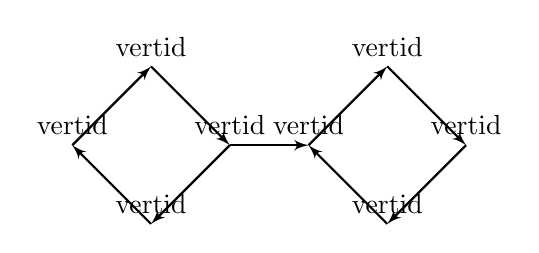
\begin{tikzpicture}
\tikzset{
    myarrow/.style={->, >=latex', thick},
}
\newcounter{vertid}
\setcounter{vertid}{1}
\foreach \x in {0,3}
{
	\draw [myarrow] (\x+1,0) node[above]{\countervalue{vertid}}--(\x+0,1);
	\draw [myarrow] (\x+0,1) node[above]{\countervalue{vertid}}--(\x+1,2);
	\draw [myarrow] (\x+1,2) node[above]{\countervalue{vertid}}--(\x+2,1);
	\draw [myarrow] (\x+2,1) node[above]{\countervalue{vertid}}--(\x+1,0);
};
\draw[myarrow] (2,1) -> (3,1);
\end{tikzpicture}
\quad
\begin{tikzpicture}
\tikzset{
    myarrow/.style={->, >=latex', thick},
}
%\newcounter{vertid}
\setcounter{vertid}{1}
	\draw [myarrow] (1,0) node[above]{\countervalue{vertid}}
	--(0,1.38);
	\draw [myarrow] (0,1.38) node[above]{\countervalue{vertid}}
	--(1,2.76);
	\draw [myarrow] (1,2.76) node[above]{\countervalue{vertid}}
	--(2.62,2.2);
	\draw [myarrow] (2.6,2.2) node[above]{\countervalue{vertid}}
	--(2.6,0.5);
	\draw [myarrow] (2.6,0.5) node[above]{\countervalue{vertid}}
	--(1,0);

\foreach \x in {6.24}
{
	\draw [myarrow] (\x-0,1.38) node[above]{\countervalue{vertid}}
	--(\x-1,0);
	\draw [myarrow] (\x-1,2.76) node[above]{\countervalue{vertid}}
	--(\x-0,1.38);
	\draw [myarrow] (\x-2.62,2.2) node[above]{\countervalue{vertid}}
	--(\x-1,2.76);
	\draw [myarrow] (\x-2.6,0.5) node[above]{\countervalue{vertid}}
	--(\x-2.6,2.2);
	\draw [myarrow] (\x-1,0) node[above]{\countervalue{vertid}}
	--(\x-2.6,0.5);

	\draw [myarrow] (2.6,0.5) -- (\x-2.6,0.5);
	\draw [myarrow] (\x-2.6,2.2) -- (2.6,2.2);

};
\end{tikzpicture}

\centering
\begin{tikzpicture}
\tikzset{
    myarrow/.style={->, >=latex', thick},
}
%\newcounter{vertid}
\setcounter{vertid}{1}
	\draw [myarrow] (1,0) node[above] (A) {\countervalue{vertid}}
	--(0,1.38);
	\draw [myarrow] (0,1.38) node[above] (B) {\countervalue{vertid}}
	--(1,2.76);
	\draw [myarrow] (1,2.76) node[above] (C){\countervalue{vertid}}
	--(2.62,2.2);
	\draw [myarrow] (2.6,2.2) node[above]{\countervalue{vertid}}
	--(2.6,0.5);
	\draw [myarrow] (2.6,0.5) node[above]{\countervalue{vertid}}
	--(1,0);

	\path [myarrow] (A) edge [loop below] (A);
	\path [myarrow] (B) edge [loop left] (B);
	\path [myarrow] (C) edge [loop above] (C);

\foreach \x in {6.24}
{
	\draw [myarrow] (\x-0,1.38) node[above] (E) {\countervalue{vertid}}
	--(\x-1,0);
	\draw [myarrow] (\x-1,2.76) node[above](F){\countervalue{vertid}}
	--(\x-0,1.38);
	\draw [myarrow] (\x-2.62,2.2) node[above]{\countervalue{vertid}}
	--(\x-1,2.76);
	\draw [myarrow] (\x-2.6,0.5) node[above] {\countervalue{vertid}}
	--(\x-2.6,2.2);
	\draw [myarrow] (\x-1,0) node[above](D) {\countervalue{vertid}}
	--(\x-2.6,0.5);

	\draw [myarrow] (2.6,0.5) -- (\x-2.6,0.5);
	\draw [myarrow] (\x-2.6,2.2) -- (2.6,2.2);

	\path [myarrow] (D) edge [loop below] (D);
	\path [myarrow] (E) edge [loop right] (E);
	\path [myarrow] (F) edge [loop above] (F);
}
\end{tikzpicture}
\caption{{\small In the first example, we can see that the only cycle cover is 
\texttt{(1,2,3,4),(5,6,7,8)}. For the second one also there is only one
cycle cover, namely \texttt{(1,2,3,4,5),(10,9,8,7,6)}.
The third is a modified version of the second example. Now there are
\emph{two} cycle covers namely, \texttt{\{(1,2,3,4,5),(10,9,8,7,6)\},
\{(1),(2),(3),(6),(7),(10),(4,5,9,8)\}}}.
}
\end{figure}

We are now set to give a characterisation of permanent over matrices in 
$\Z^{n \times n}$, which we will be crucially using in the next lecture.

\begin{lemma}
Let $A \in \Z^{n \times n}$. Let $G$ be the directed weighted graph obtained
by interpreting $A$ as the weighted adjacency matrix of $G$, i,e. 
\[|V(G)| = n,\] \[ \forall 1 \le i,j \le n, wt(i, j) = w \iff A_{i,j} = w \]
then
\[ \perm(A) = \sum_{\substack{\calC \in Cyclecover(G)}} wt(\calC) \]
\end{lemma}
\begin{proof}
We show that corresponding to every permutation $\sigma \in S_n$, there is a
unique cycle cover $\calC$. That is,
\[ \prod_{\substack{i=1}}^n A_{i,\sigma(i)} = k \iff \exists~\calC \text{ such
that } wt(\calC) = k \]

($\Leftarrow$) Suppose there is a cycle cover $\calC$ such 
that $wt(\calC) = k$. Without loss of generality assume $k \not = 0$. 
(If $k=0$, then one of the edges is not  present and hence no cycle cover is 
possible using the edges in $\calC$).  
Now we can define a permutation to be $\sigma(i) = j~\forall (i,j)\in \calC$.
Since $\calC$ covers all vertices, $\sigma$ is defined for all $\{1,2,\ldots,
n\}$ and since $\calC$ is composed of cycles, every $(i,j)$ will be unique.
Hence the map $\sigma$ will be bijective and is a valid permutation in $S_n$.
Also $\prod_{i=1}^n A_{i,\sigma(i)} = \prod_{(i,j) \in \calC} wt(i,j) =
wt(\calC) = k$.

($\Rightarrow$) Similarly, given a permutation $\sigma$ such that $\prod_{i=1}^n
A_{i,\sigma(i)} = k$, we construct a cycle cover as follows.

If $k=0$, then there is no cycle cover possible with the given permutation
since a zero weight edge is appearing. Hence let $k \not = 0$. Fix an $i\in
\{1,2,\ldots,n\}$. Consider the sequence $(i, \sigma(i), \sigma^2(i), \ldots,
\sigma^n(i))$ where $\sigma^i$ for $i \ge 0$ is obtained by applying $\sigma$
function $i$ times. It can be seen by pigeon hole principle that atleast one
values in the sequence must repeat (since, $\sigma$ is defined on $n$ 
terms and there are $n+1$ terms in the sequence). Without loss of generality, 
let $\sigma^l(i)$ and $\sigma^m(i)$ repeat with $ 0 \le l < m \le n$. 
Since all the weights  are non-zero, the vertices 
$\sigma^l(i), \sigma^{l+1}(i), \ldots, \sigma^m(i) = \sigma^l(i)$ have 
edges between them and clearly forms a cycle. We can find
all the cycles by repeating this process for various values of $i$. 
Note that since $\sigma$ is a permutation, the cycles obtained will be disjoint 
and will cover the entire graph.

Now taking sum over all permutations on both sides proves the claim.
\end{proof}

Using this result the following observation (which is left as an exercise) can
also be made.
\begin{observation}
For $A \in \Z^{n\times n}$ computing permanent of $A$ is in $\FP^{\#\P}$.
\end{observation}

\newpage 
\newcommand{\sP}{\#\P} %% The class #P as it is not defined in complexity.sty
\Lecture{Akshay Degwekar, Devanathan.T}{Jan 17, 2012}{8}{Permanent Computation is \sP-Complete}

\newcommand{\per}{{\sf Per}} % Permanent is defined as an operator.
\newcommand{\wt}{{\sf Weight}} % Weight is defined as an operator.
\newcommand{\integer}{\mathbb{Z}}

In this lecture, we define the permanent of a matrix and study the complexity of computing the permanent for various classes of matrices. Finally we prove a theorem by Valiant that $\per(A)$ is \sP-Complete.

\begin{definition}
\textbf{Permanent } Given a matrix $A_{n \times n}$, Let $S_n$ be the set of all permutations of $[n]$. Then
\begin{equation}
\per(A) = \sum_{\sigma \in S_n } \prod_{i=1}^n A_{i,\sigma(i)} 
\end{equation}
\end{definition}

Earlier, we have seen a characterization of the permanent as the number of perfect matchings in a graph G. To prove the result, we characterize the permanent using \textbf{Cycle Covers}.

\begin{definition}
\textbf{Cycle Cover } A Cycle Cover $C$ of a directed graph G is a set of pairwise disjoint simple cycles such that each vertex lies in exactly one cycle in $C$.

Note that we allow self-loops as simple cycles.

\xymatrix{
		  & 3 \ar[dr]&	            &   	&	7\ar[dr] \\
2 \ar[ur]& 		 &4\ar[dl]\ar[r]&6\ar[ur]  && 8\ar[dl] \\
&1 \ar[ul]&&&5\ar[ul]&\\}
Has a cycle cover $\big{\{}\{1,2,3,4\},\{5,6,7,8\}\big{\}}$.

\begin{definition}
\textbf{Weight of a Cycle Cover} Given a Graph $G(V,E)$, let $C={C_1, C_2, \dots C_l}$ be any cycle cover
\begin{equation}
\textbf{Weight of Cycle - } \wt(C_i) = \prod_{e\in E}w(e)
\end{equation}
\begin{equation}
\textbf{Weight of Cycle Cover - } \wt(C_i) = \prod_{c\in C}\wt(c)
\end{equation}
\end{definition}


%%That is, In a graph $G(V,E)$, $C = {C_1, C_2, \dots C_l}$ is a cycle cover iff $\forall i,j \quad C_i\cap C_j = \phi$ and $v\in V, \, \exists ! j $ such that $•$ $C_j$ is a 

\end{definition}

\begin{lemma}
Let $G(V,E)$ be a graph with adjacency matrix $A$. 
$A \in \mathbb{Z}^{n\times n}$. Then 
\begin{equation}
	\per(A) = \sum_{\substack{C \text{ is a} \\ \text{Cycle Cover}}} \wt(C)
\end{equation}
\end{lemma}
\begin{proof}
Consider a single term from the permanent - $\sum^n_{i=1}A_{i,\sigma(i)}$.

We can view $\sigma$ as a cycle cover as follows. 

First we decompose $\sigma$ into cycles of the form $a, \sigma(a), \sigma^2(a)\dots \sigma^k(a) = a$. 

Now each cycle in the permutation can be viewed as a cycle in the graph G. The edges being $\big{\{} (1, \sigma(1)),(2, \sigma(2)), \dots (n, \sigma(n)) \big{\}}$.

This is the required cycle cover. There is a bijective correspondence between the permutations and the cycle covers. 

Note, some of the cycle covers generated from permutation might not be valid that is some edges are absent. In that case, we just see that their weight is 0 as $A_{i,j} = 0$ for the edge $(i,j)$ not present. 

And in the case that it is a valid cover, $\wt(C) = \prod_{i\in[n]}A_{i,\sigma(i)}$, because both of them are exactly the product of the corresponding edges.

This completes the proof.
\end{proof}

%%%%%%%%%%%%%%%%Some explanation and notes are required here.

\begin{exercise}
Let $\mathbb{Z}_+$ denote the non negative integers.
Using the previous construction involving Weighted Matching, 
show that for $A\in \mathbb{Z}_{+}^{n\times n}, \per(A)\in \FP^\sP$.

 This problem is also a part of the first problem set.
\end{exercise}


\begin{exercise}
Is the reduction from $\SAT$ to $3\SAT$ parsimonious? If not, show that $\#3\SAT$ is $\sP-complete$. 
\end{exercise}

%%%%%Some embellishment might be needed here.
Now, we move towards the final part of the lecture - the result by Valiant, that $Per$ is $\sP-Hard$. The proof given here is due to Del.... %add the citations here for both the papers.
We will show this by using a gadget construction.

\begin{theorem}
$\#3\SAT\in \FP^{\per}$
\end{theorem}
\begin{proof}
Consider a formula $\phi $ in $3\SAT$. $\phi = C_1\wedge C_2 \dots C_m$ where $C_i = l_{i,1}\vee l_{i,2} \vee l_{i,3}$.

We will construct a directed graph $G$ such that $A_G$ is the adjacency matrix of $G$, such that $A_G \in \{-1,0,1\}^{n\times n}$ and also, $\per(A_G)=(-2)^k(\#\phi)$ where $(\#\phi)$ is the number of satisfying assignments of $\phi$ and $k$ is a quantity that we specify later.

\begin{lemma}
Let $\#x$ be the number of times a variable $x$ occurs in $\phi$. 

Then $\phi$ can be converted to $\phi'$ such that $\forall x$, $k = \#x=\# \overline{x}$ and $\#phi = \# phi'$
\end{lemma}

\begin{proof}
 We first observe that if $\# x \not = \# \overline{x}$. Then this imbalance can be removed by adding terms of the form $(x\vee x\vee \overline{x})$ and/or $(x\vee \overline{x}\vee \overline{x})$ because they add or decrease the relative number of $x$ compared to $\overline{x}$.
 
 Now, we assume that $\forall x, \#x = \# \overline{x}$.
 Now to compensate for relative differences between $x, y$ we add terms of the form $(x\vee \overline{x}\vee \overline{y})\wedge (x\vee \overline{x}\vee \overline{y})$ to increase the number of $x$ and the other way to decrease.
 
 And we just note that the number of solutions is invariant because each of the added terms are always true.
 
 This completes the lemma.
 \end{proof}
  
  We will be constructing the graph from three gadgets - Variable Gadget, Clause Gadget and the Equality Gadget.

%%% The gadgets  
\begin{figure}[h!]
\centering
%%%%%%%Variable Gadget
\begin{subfigure}[b]{0.3\textwidth}
\xymatrix{ 
	{\bullet}  \ar @/_/ [dd]_x  \ar @/^/ [dd]^{\overline{x}} \\ \\
	{\bullet} \ar [uu]}
	\caption{Variable Gadget}
\end{subfigure} 
%%%%%%%Clause Gadget
\begin{subfigure}[b]{0.3\textwidth}
\centering
 \xymatrix{ 
	 & {\bullet}  \ar @/^/ [d]   \ar @/_/ [ddl]_{\overline{l_1}} & \\ 
	 & {\bullet}  \ar @/^/ [u]  \ar @/^/ [dl]  \ar @/^/ [dr] & \\
{\bullet}\ar @/_/ [rr]_{\overline{l_3}} \ar @/^/ [ur] & & {\bullet}  \ar @/^/ [lu] \ar @/_/ [uul]_{\overline{l_2}} \\	
	}
	\caption{Clause Gadget}
\end{subfigure}
%%%%%%%Equality Gadget
\begin{subfigure}[b]{0.3\textwidth}
\centering
 \xymatrix{ 
	\ar @/_/[ddr] & & {\bullet} \ar@(ul,ur)^{-1} \ar @/_/[ddr] \ar @/_/ [ddl]& & \ar @/^/[ddl] \\ 
	\\
	\ar @/^/[r] & {\bullet}  \ar@(dl,dr)_{1}\ar @/_/ [uur]  \ar @/_/ [rr] & &  {\bullet}  \ar @/_/[uul]  \ar @/_/[ll] \ar@(dl,dr)_{1} & \ar @/_/[l] }
	
	\caption{Equality Gadget}
\end{subfigure}
\caption{The Gadgets}
\label{fig1Gadgets}
\end{figure}

Now, we consider the construction of the graph.

For each variable pair $(x, \overline{x})$ we have one variable gadget. Each clause has a Clause Gadget and the equality gadget is used to join each variable with all the clauses the variable is in.

The equality gadget is represented as a black box as follows -
\begin{figure}[h!]
\centering
\begin{subfigure}[b]{0.3\textwidth}
\centering
 \xymatrix{ 
	\ar @/_/[ddr] & & {\bullet} \ar@(ul,ur)^{-1} \ar @/_/[ddr] \ar @/_/ [ddl]& & \ar @/^/[ddl] \\ 
	\\
	\ar @/^/[r] & {\bullet}  \ar@(dl,dr)_{1}\ar @/_/ [uur]  \ar @/_/ [rr] & &  {\bullet}  \ar @/_/[uul]  \ar @/_/[ll] \ar@(dl,dr)_{1} & \ar @/_/[l] }
	
	\caption{Equality Gadget}
\end{subfigure}
\begin{subfigure}[b]{0.3\textwidth}
\centering
\xymatrix{ 
	\ar @/_/[drr] & \ar @{-} [rrr] \ar @{-} [dd]& & &\ar @{-} [dd] & \ar @/^/[dll]\\
 & & \ar @/_/[dll]&\ar @/^/[drr] & & \\
 & \ar @{-} [rrr]& & & &\\
}	
	\caption{Equality Gadget Representation}
\end{subfigure}
\caption{Equality Gadget Blackbox representation}
\label{fig:EqBlackbox}
\end{figure}

The way we connect a variable and a clause is shown in the next figure. Here $\overline{x}$ is the literal $l_1$ in the clause. 

\begin{figure}[h!]
\centering

\begin{subfigure}[b]{0.3\textwidth}
\centering
\xymatrix{ 
{a}  \ar @/_/ [dd]_x  \ar @/_/[drr]^{u} & \ar @{-} [rrr] \ar @{-} [dd]& & &\ar @{-} [dd] &  & 
{\bullet} \ar @/^/[dlll]^{u'}  \ar @/^/ [d] &  \\ 
 & & \ar @/_/[dll]^{v} &\ar @/^/[drr]^{v'} & &  &  
{\bullet}  \ar @/^/ [u]  \ar @/^/ [dl]  \ar @/^/ [dr] & \\
{b} \ar [uu] & \ar @{-} [rrr]& & & &
{\bullet} \ar @/_/ [rr]^{\overline{l_3}} \ar @/^/ [ur] & & {\bullet} \ar @/_/ [uul]^{\overline{l_2}}  \ar @/^/ [lu] \\	
}	
\end{subfigure}
\caption{Connection between variables and clauses.}
\label{VarClauseConnection}
\end{figure}

When the same variable appears in multiple clauses, we split the edge representing the variable and attach multiple equality gadgets. The next figure shows the split.

\begin{figure}[ht!]
\begin{subfigure}[b]{0.3\textwidth}
\xymatrix{ 
	{\bullet}  \ar @/_/ [ddd]_{\overline{x}}  \ar @/_/ [dr] & & & &  \\ 
& Equality Gadget \ar @/_/ [d] \ar @/_/ [rr] & & Clause Gadget \ar @/_/ [ll]& &\\
& Equality Gadget  \ar @/_/ [dl] \ar @/_/ [rr] & & Clause Gadget \ar @/_/ [ll]& & \\
	{\bullet} \ar [uuu]}
	\label{fig:subfigure1}
\end{subfigure}
	\caption{One variable occurring in multiple clauses.}
\end{figure}

This essentially completes the construction. We will prove the correctness of the construction in a series of claims.
\begin{claim}
Any cycle cover can either use the edge $x$ or $\overline{x}$ in the variable gadget, but not both.
\end{claim}
\begin{proof}
If a cycle cover used both the edges, then the vertices would be covered twice. 
\end{proof}

\begin{claim}
Each assignment corresponds to atleast one cycle cover. 
\end{claim}
\begin{proof}
For each variable, choose $x$ or $\overline{x}$ based on the assignment. And for each clause choose the cycle $l_1 \rightarrow l_2 \rightarrow l_3$ and choose self-loops everywhere else.
\end{proof}

We will derive a much precise correspondence in the remaining proof.


\begin{claim}
In any cycle cover C, either both $u,v$ are used, or neither $u,v$ are used.
\end{claim}
\begin{proof}
The proof is just a verification, We see in \ref{VarClauseConnection} that if the edge $u$ is used, edge $(b,a)$ will have to be used, and to complete a cycle, we will need $v$ to complete the cycle as the edge $x$ cannot be used. 

The proof holds unmodified for edges $u',v'$ too.
\end{proof}

\begin{claim}
If both $u,v$ and $u',v'$ edges are used in the cycle cover, then the $-1$ valued self-loop has to be chosen in the cycle cover. 
\end{claim}

\begin{claim}
If edges $u,v$ are used while $u',v'$ are not used, the corresponding Cycle Covers contribute weight 0.
\end{claim}
\begin{proof}
We just observe that there are two components one contributing $+1$ and the other as $-1$ in the cycle weight. Cycle covers are marked in double lines.

\begin{figure}[H]
\begin{subfigure}[b]{0.3\textwidth}
\centering
 \xymatrix{ 
	\ar @{=>} @/_/[ddr]^{u}  & & {\bullet} \ar@(ul,ur)^{-1} \ar @{=>}@/_/[ddr] \ar   @/_/ [ddl]& & \ar @/^/[ddl]_{u'} \\ 
	\\
	\ar @{<=} @/^/[r]_{v} & {\bullet}  \ar@(dl,dr)_{1}\ar  @/_/ [uur]  \ar @/_/ [rr] & &  {\bullet}  \ar @{=>} @/_/[uul]  \ar @/_/[ll] \ar@(dl,dr)_{1} & \ar @/_/[l]^{v'} }
	\caption{Weight +1}
\end{subfigure}
\begin{subfigure}[b]{0.3\textwidth}
\centering
 \xymatrix{ 
	\ar @{=>}@/_/[ddr]^{u}  & & {\bullet} \ar@{=>}@(ul,ur)^{-1} \ar @/_/[ddr] \ar @/_/ [ddl]& & \ar @/^/[ddl]_{u'} \\ 
	\\
	\ar @{<=}@/^/[r]_{v} & {\bullet}  \ar@(dl,dr)_{1}\ar @/_/ [uur]  \ar @/_/ [rr] & &  {\bullet}  \ar @/_/[uul]  \ar @/_/[ll] \ar@{=>}@(dl,dr)_{1} & \ar @/_/[l]^{v'} }
	\caption{Weight -1}
\end{subfigure}
\caption{Only one of the two sets of edges are present}
\end{figure}
\end{proof}


\begin{claim}
If both $u,v$ and $u',v'$ are not used, then the Cycle Covers have a contribution of 2 from this gadget. 
\end{claim} 
\begin{proof}
The figure \ref{Fig6} contains all the possible cycle covers of the gadget. Their contributions sum upto 2.
\begin{figure}[h]
\begin{subfigure}[b]{0.3\textwidth}
\centering
 \xymatrix{ 
	\ar  @/_/[ddr]^{u}  & & {\bullet} \ar @{=>}@(ul,ur)^{-1} \ar @/_/[ddr] \ar   @/_/ [ddl]& & \ar @/^/[ddl]_{u'} \\ 
	\\
	\ar  @/^/[r]_{v} & {\bullet}  \ar @{=>}@(dl,dr)_{1}\ar  @/_/ [uur]  \ar @/_/ [rr] & &  {\bullet}  \ar @/_/[uul]  \ar @/_/[ll] \ar @{=>}@(dl,dr)_{1} & \ar @/_/[l]^{v'} }
	\caption{Weight -1}
\end{subfigure}
\begin{subfigure}[b]{0.3\textwidth}
\centering
 \xymatrix{ 
	\ar @/_/[ddr]^{u}  & & {\bullet} \ar@{=>}@(ul,ur)^{-1} \ar @/_/[ddr] \ar @/_/ [ddl]& & \ar @/^/[ddl]_{u'} \\ 
	\\
	\ar @/^/[r]_{v} & {\bullet}  \ar@(dl,dr)_{1}\ar @/_/ [uur]  \ar@{=>}@/_/[rr] & &  {\bullet}  \ar @/_/[uul]  \ar@{=>}@/_/[ll] \ar@(dl,dr)_{1} & \ar @/_/[l]^{v'} }
	\caption{Weight -1}
	\end{subfigure}
\begin{subfigure}[b]{0.3\textwidth}
\centering
 \xymatrix{ 
	\ar  @/_/[ddr]^{u}  & & {\bullet} \ar @(ul,ur)^{-1} \ar @{=>}@/_/[ddr] \ar   @/_/ [ddl]& & \ar @/^/[ddl]_{u'} \\ 
	\\
	\ar  @/^/[r]_{v} & {\bullet}  \ar @{=>}@(dl,dr)_{1}\ar  @/_/ [uur]  \ar @/_/ [rr] & &  {\bullet}  \ar @{=>}@/_/[uul]  \ar @/_/[ll] \ar @(dl,dr)_{1} & \ar @/_/[l]^{v'} }
	\caption{Weight 1}
\end{subfigure}	
\begin{subfigure}[b]{0.3\textwidth}
\centering
 \xymatrix{ 
	\ar  @/_/[ddr]^{u}  & & {\bullet} \ar @(ul,ur)^{-1} \ar @/_/[ddr] \ar@{=>}@/_/ [ddl]& & \ar @/^/[ddl]_{u'} \\ 
	\\
	\ar  @/^/[r]_{v} & {\bullet}  \ar@(dl,dr)_{1}\ar  @{=>}@/_/ [uur]  \ar @/_/ [rr] & &  {\bullet}  \ar @/_/[uul]  \ar @/_/[ll] \ar @{=>}@(dl,dr)_{1} & \ar @/_/[l]^{v'} }
	\caption{Weight 1}
\end{subfigure}	
\begin{subfigure}[b]{0.3\textwidth}
\centering
 \xymatrix{ 
	\ar  @/_/[ddr]^{u}  & & {\bullet} \ar @(ul,ur)^{-1} \ar @/_/[ddr] \ar@{=>}@/_/ [ddl]& & \ar @/^/[ddl]_{u'} \\ 
	\\
	\ar  @/^/[r]_{v} & {\bullet}\ar@(dl,dr)_{1}\ar@/_/ [uur]\ar@{=>}@/_/ [rr] & &  {\bullet}  \ar@{=>}@/_/[uul]  \ar @/_/[ll] \ar @(dl,dr)_{1} & \ar @/_/[l]^{v'} }
	\caption{Weight 1}
\end{subfigure}	
\begin{subfigure}[b]{0.3\textwidth}
\centering
 \xymatrix{ 
	\ar@/_/[ddr]^{u}  & & {\bullet} \ar@(ul,ur)^{-1} \ar@{=>}@/_/[ddr] \ar@/_/ [ddl]& & \ar @/^/[ddl]_{u'} \\ 
	\\
	\ar  @/^/[r]_{v} & {\bullet}\ar@(dl,dr)_{1} \ar@{=>}@/_/[uur] \ar@/_/[rr] & &  {\bullet}\ar@/_/[uul]  \ar@{=>}@/_/[ll] \ar@(dl,dr)_{1} & \ar@/_/[l]^{v'} }
	\caption{Weight 1}
\end{subfigure}	
\caption{The weights sum upto 2}
\label{Fig6}
\end{figure}
\end{proof}

\begin{claim}
	Weight of each cycle cover is $(-2)^{kn}$
\end{claim}
\begin{proof}
We want to claim that if a variable $x$ is assigned value $1$, then all the equality gadgets for $x$ will contribute $1$ to the weight because $u,v$ and $u',v'$ will both be a part of the cycle cover for each of the gadgets, if just one pair is in the cycle cover, we have seen that those covers would contribute 0 to the weight. 

Also, the gadgets that correspond to $\overline{x}$ will not have either $u,v$ or $u',v'$ being used - because, $u,v$ cannot be used as $x$ edge will be used, hence $\overline{x}$ cannot be used. Now, if $u',v'$ are used, those cycles will have 0 weight as seen in the observation.

So, the only possibility there is both $u,v$ and $u',v'$ are not used. In that case, the contribution would be $2$ for each gadget. As there are $k$ such gadgets, we will have a contribution of $2^k$ from these. 

So, multiplying them would give us, that each variable pair $x,\overline{x}$ contribute exactly $(-2)^k$ to the weight. Hence the cycle cover would have a weight of exactly $(-2)^{kn}$.

So, We sum them up over all the possible assignments to get the required result. This completes the proof.

\end{proof}

So, we have the result -
\begin{equation}
{\sum_{\text{C is a Cycle Cover}} \wt(C) }= \per_{-1,0,1}(A)
\end{equation}

Hence computing $\#\SAT$ reduces to computing $\per_{-1,0,1}$. This completes the proof. 
\end{proof}

Now we will first show that $\per_{-1,0,1}$ reduces to $\per_{0,1,\dots n}$ and finally show that $\per_{0,1,\dots n}$ reduces to $\per_{0,1}$ and hence completing the theorem.

\begin{theorem}
$\per_{-1,0,1} \in \FP^{\per_{0,1,\dots n}}$.
\end{theorem}
\begin{proof}
 The first thing we observe is that all the -1 terms in the adjacency matrix $A$ represent self-loops because in the construction, $-1$ was the edge weight of only one self-loop.
 
 Consider $\per(A)$ as a polynomial in $x$ where each $-1$ is replaced by $x$ denoted by $p(x)$ 
 
 Now we just observe that, using ${\per_{0,1,\dots n}}$ as an oracle, we can find $p(0), p(1), ... p(n)$. Also, degree of p $\leq n$ because x occurs only in the diagonal entries, hence only n $x $ can be present. 
 
 So, now we just use Lagrange Interpolation to find the polynomial $p$. This can be done in poly time. Once this is done, $\per_{-1,0,1}(A) = p(-1)$, which can be computed easily.
 
 This completes the reduction.
\end{proof}

In the final reduction, we show that $\per_{0,1,\dots n} \in \FP^{\per_{0,1}}$, and that $\per_{0,1}$ is as hard as the other $\per$ computations. 

\begin{theorem}
$\per_{0,1,\dots n} \in \FP^{\per_{0,1}}$
\end{theorem}
\begin{proof}
This proof involves substituting the $-1$ self-loop with a gadget so that we can compute the values of the polynomial $p(x)$ at points $x=0, x=1, \dots x=n$.

The gadget we use is - 
Consider any $a = (a_k, a_{k-1}\dots a_{0})_2$ in base $2$ where $a\in \{0, 1, \dots n\}$. Now we want to replace the self-loop of weight $a$ with the gadget, so that the gadget contributes exactly $k$ weight to the Cycle cover. 

\begin{figure}[ht!]
\xymatrix{
\ar[r]^{1} & \ar@/^/[d]^{a_0} \ar@/_/[r]^{1} \ar@/^/[r]^{1} & \ar@(ul,ur) \ar@/^/[dl]^{a_1} \ar@/_/[r]^{1} \ar@/^/[r]^{1}  & \ar@(ul,ur) \ar@/^/[dll]^{a_2} \ar@[--][r] & \ar@(ul,ur) \ar@/^/[dlll]^{a_{k-1}}   \ar@/_/[r]^{1} \ar@/^/[r]^{1} & \ar@(ul,ur) \ar@/^/[dllll]^{a_{k}} \\ 
& \ar[ul]^{1} & & \\
}
\end{figure}

The gadget has precisely $n$ cycles of weight $1$ each. This gadget can be used to replace the self loop and then query the $\per_{0,1}$ oracle. 

This completes the reduction. Hence proved.
\end{proof}


\newpage 

\newcommand{\paths}[2]{\ensuremath{\#paths_{M}(x)}}
\newcommand{\acc}[2]{\ensuremath{\#acc_{M}(x)}}
\newcommand{\rej}[2]{\ensuremath{\#rej_{M}(x)}}
\newcommand{\err}[2]{\ensuremath{\#err_{M}(x)}}

\newcommand{\ParityP}{\ensuremath{\oplus\P}}

% \newcommand{\iff}{\LeftRightarrow}


\Lecture{Balagopal}{23 Jan, 2012}{09}{Probabilistic TMs and Randomized Algorithms}
%\theme{}
%\lectureplan{}

\section{Review of Branching machines}

A branching machine is a machine that is allowed to make non-deterministic guesses while computation. This is 
a generalization of NTMs where the branching machine accepts iff at least one path accepts. Similarly we can think of 
various definitions of acceptance each of them leading to a (possibly) new complexity class. For example, \PP\ is defined as the class 
which has a branching machine where more than half of the paths accept. \ParityP\ is defined as the class where each language has a 
branching machine in which an odd number of paths accept if $x \in L$. Similarly we can think of every branching machine as computing 
a function $f(x)$ where $f(x)$ is defined as the number of accepting paths of $M$ on $x$.

\textbf{Question. } How is \ParityP\ related to \P\ , \NP\ , \PSPACE\ , and \PP\ ?

We will come back to answer this question, and show that $\NP$ can be
{\em almost} solved in $\P$ if $\ParityP$ can be solved in $\P$. The
{\em almost} here will refer to possibility of error by the algorithm
in the decision. We will now do a systematic formal study of
randomized algorithms (algorithms which may make an error but with low
probability). We introduce these from the branching machine
perspective that we have seen so far.

\section{Characterizing Randomized Algorithms}

We are going to characterize randomized algorithms using branching machines that we 
defined previously.

Consider a branching machine $M$ for the language $L$. If $x \in L$ call all paths of $M$ that 
reject as erroneous. If $x \notin L$ call all paths of $M$ that accept as erroneous. Intuitively, 
we want the erroneous paths to be as small as possible. We use the following notations for counting 
paths with specific properties for a branching machine $M$.

\begin{description}
\item[$\paths{M}{x}$] Total number of paths of $M$ on $x$

\item[$\acc{M}{x}$] Total number of accepting paths of $M$ on $x$

\item[$\rej{M}{x}$] Total number of rejecting paths of $M$ on $x$

\item[$\err{M}{x}$] Total number of erroneous paths of $M$ on $x$
\end{description}

We defined class \PP\ as the set of languages $L$ with branching machines 
satisfying the following property.

\begin{eqnarray*}
x \in L &\implies& P(A \textrm{ accepts } x) > 1/2 \\
x \notin L &\implies& P(A \textrm{ rejects } x) \geq 1/2
\end{eqnarray*}

To connect the notion of a branching program and a randomized algorithm, we have to make sure 
that all paths of the branching machine are of the same length (i.e., the computation tree is a full 
binary tree). This can be done by a construction similar to the one used to do this while defining \#\P.
However, when a path is extended by branching it yields multiple paths. We must ensure that the error probabilities are not 
increased during this process.
Note that this is different from what we did while defining \#\P. 
The goal there was to preserve the count (Number of accepting paths). 
The goal here is to keep the error probability (which depends on the relative number of accepting and rejecting paths) the same.

Now consider a randomized algorithm $A$ that chooses one path of $M$ uniformly at random and 
executes it (This shows that there is a randomized algorithm corresponding to every branching machine). 
Clearly

\begin{equation}
x \in L \iff \err{M}{x} \leq \frac{1}{2} \paths{M}{x}
\end{equation}


We see that the probability of $A$ making an error is at most 1/2. But this can be 
achieved by a trivial randomized algorithm that flips a coin and determines the result according 
to the outcome of the coin flip. So the class \PP\ is not a good candidate for formally capturing 
``good'' randomized algorithms.

What we want is the error probability to be bounded away from $1/2$. If $\err{M}{x} < \frac{1}{4} \paths{M}{x}$, then 
certainly the corresponding randomized algorithm is better than a trivial one.

We will now work towards defining a problem for which there is an efficient (poly time) randomized algorithm but for which 
no poly time deterministic algorithm is known. This gives reason to study randomized algorithms formally.


\section{Polynomial Identity Testing}

This problem has its roots in the simple high school
arithmetic. Suppose we are given a polynomial in a complicated form
where the monomials may repeat with arbitrary coefficients etc. We
want to find out if the coefficient of the monomials cancel out to
zero. This in effect is testing whether the polynomial is the zero
polynomial, and equivalenty it is testing if the polynomials evaluates
to zero on all substitutions of the variable from the underlying field
$\mathbb{F}$.

How are we given the polynomial? This indeed is going to have effect
on the complexity of the problem.  Let us start with the high school
arithmetic again. Suppose we are given it in the monomial form (though
some monomials may repeat) along with their coefficients. To solve the
problem, it suffices to check, for each monomial whether the
coefficient in its various appearences is adding up to zero. Given the
explicit representation at the input, this is very easy to do by
simply going over the input for each monomial. Hence this can be done
in time polynomial in the input.

What if the polynomial is not given that explicity. What is the most
implicit form that we can think of? A black box which evaluates the polynomial.
That is, we have an oracle $p$ when given input $a$ returns $p(a)$, the value of polynomial 
at $a$.

%The aim is to test whether the input polynomial is identically 0 (The zero polynomial). If the polynomial 
%is given as monomials, then we can do this in {\tt poly} time. But what if the input polynomial is given in 
%$blackbox form. 

Assume that we are also given an upper bound on the degree of the
polynomial $deg(p) \leq d$.  Indeed, we do not have access to the
actual polynomial except through the blackbox. We have to use some
property of the degree $d$ polynomials. The most obvious one is the
number of points in which they can evaluate to zero. Based on this thought, 
the following deterministic algorithm solves the problem.

\begin{figure}[ht]
{\tt \obeyspaces \obeylines
1. Choose $d + 1$ different points $a_1 , \ldots , a_{d+1}$.
2. Call the oracle $d+1$ times to evaluate $p(a_1), \ldots , p(a_{d+1})$.
3. If all calls returned 0 accept else reject.
}
\caption{A deterministic algorithm for univariate polynomial identity testing}
\end{figure}

If $p$ were really 0 then all calls will return 0 and we will definitely accept. If $p$ were not 
0, then at most $d$ calls can return 0 since a polynomial with degree at most $d$ has at most $d$ 
roots. Hence if $p \neq 0$, then our algorithm will definitely reject.

Now let us think about the problem when $p$ is a multivariate
polynomial. The previous assertion that a degree $d$ polynomial has at
most $d$ roots no longer holds. To see this, consider the degree 2
polynomial $p(x_1, x_2) = x_1 x_2$. This has an infinite number of
roots $x_1 = 0, x_2 \in \mathbb{F}$, where $\mathbb{F}$ is the
(possibly infinite) field over which $p$ is defined.  We can work
around this problem by considering a finite subset of the field, say
$S = \{ 0, \ldots ,10 \}$. The polynomial $p$ has $19$ zeroes. So if
$x_1, x_2$ is chosen uniformly at random from $S$ there is at most
$19/100$ chance that we will get a false result. As can be seen from
the above example, by making the size of $S$ arbitrarily large, we can
make the error probability arbitrarily small. But then the
disadvantage is that we will need more random bits in order to choose
an element at random from the set $|S|$, and the running time of our
algorithm will also increase.

In the next lecture, we will show that this intuition is correct by
exhibiting a low error polynomial time randomized algorithm for the
multivariate case. The question of finding a deterministic algorithm
for this problem is open. Although it looks like a simple algorithmic
problem from algebra which only mathematicians might be interested in,
there are several computational problems that can be encoded into this
form and hence can be solved efficiently if this algorithmic problem
can be solved efficiently.
 

\newpage \Lecture{Sunil K S}{Jan 24, 2012}{10}{Polynomial Identity Testing}

Towards the end of last lecture, we introduced the following problem :
{\em Given a polynomial $p$, test if it is identically zero}. That is,
do all the terms cancel out and become the zero polynomial. Described
as a language :
$$\textrm{\sc PIT}=\{ p ~|~p \equiv 0\}$$
We also saw some easy cases of the problem:
\begin{enumerate}
\item When it is given as a sum of monomials: Given $p$, run over the
  input to figure out the coefficient of each monomial, and if all of
  them turn out to be zero, then report that $p$ is in {\sc PIT}. This
  algorithm runs in $O(n^2)$ time.
\item When it is given as a Black Box: In uni-variate case, check
  $p(x)$ for $d+1$ different points where $d$ is the degree bound. If
  the polynomial is not equivalent to zero, then at-least one of the
  steps gives a non-zero value. Indeed, if the polynomial is zero,
  then all the $(d+1)$ evaluations will result in a zero value. Thus
  the algorithm is correct and runs in time $O(d)$ where $d$ is the
  degree of the polynomial.
\end{enumerate}

As we observed, this strategy could not be generalized in
multi-variate case. We took an example as $p(x_1,x_2) = x_1x_2$. For
the assignment $x_1=0$, whatever $x_2$ chose, the value will always be
0. However, if $p \equiv 0$, no matter what we choose as the
substitution for $x_1$, and $x_2$, the polynomial will be identically
zero.

The strategy that we will follow is as follows: If the total degree of
the polynomial is $\leq d$, and if $S \subseteq \F$, such that
$|S|\geq 2d$, instead of picking elements arbitrarily, we pick
elements uniformly at random from $S$. Indeed, there may be many
choices for the values which may lead to zero. But how many?
%Here by increasing the size of $S$, we can improve the probability.
% IMPRECISE statement.

\begin{lemma}[Schwartz-Zippel Lemma]
Let $p(x_1, x_2, \cdots , x_n)$ be a non-zero polynomial over a field
$\mathbb{F}$. Let $S\subseteq \mathbb{F}$
$$Pr[p(\bar{a}=0]\leq \frac{d}{|S|}$$
\end{lemma}
%It also shows that the number of solutions for $P(\bar{a})$ if $\leq d|S|^{(n-1)}$.
\begin{proof}
(By induction on $n$) For $n=1$: For a univariate polynomial $p$ of
  degree $d$, there are $\leq d$ roots. Now in the worst case the set
  $S$ that we picked has all $d$ roots. Thus for a random choice of
  substitution for the variable from $S$, the probability that it is a zero of
  the polynomial $p$ is at most $\frac{d}{|S|}$.

For $n>1$, write the polynomial $p$ as a univariate polynomial in $x_1$ with coefficients as polynomials in the variables $p(x_2, \ldots, x_n)$.
$$ \displaystyle \sum_{j=0}^{d}x_1^jp_j(x_2, x_3, \ldots, x_n)$$

For example: $x_1x_2^2+x_1^2x_2x_3+x_3^2=(x_2x_3)x_1^2+(x_2^2)x_1+x_1^0(x_3^2)$.

To analyse the probability that we will choose a zero of the
polynomial (even though the polynomial is not identically zero). For a
choice of the variables as $(a_1, a_2, \cdots, a_n)\in S^n$, we ask
the question : how can $p(a_1, a_2, \cdots, a_n)$ be zero? It could be
because of two reasons:

\begin{enumerate}
\item $\forall j~:~1 \le j \le n , ~~ p_j(a_2, a_3, \ldots , a_n)=0$.
% In this case whatever $(a_2, a_3, \cdots , a_n)=0$, polynomial will be zero.
\item %$(a_2, a_3, \cdots , a_n)=0$.
Some coefficients $p_j(a_2, a_3, \ldots , a_n)=0$ are non-zero, but
the resulting univariate polynomial in $x_1$ evaluates to zero upon
substituting $x_1 = a_1$.
\end{enumerate}

Now we are ready to calculate $Pr [ p(a_1, a_2, \ldots, a_n) = 0 ]$.
%\begin{eqnarray*}
For a random choice of $(a_1, \ldots, a_n)$.
Let $A$ denote the event that the polynomial $p(a_1, \ldots, a_n) = 0$.
Let $B$ denote the event that $\forall j~:~1 \le j \le n ,~~p_j(a_2, a_3, \cdots , a_n)=0$.
Now we simply write : $Pr[A] = Pr[A \land B]+Pr[A\land \bar{B}]$.

We calculate both the terms separately: $Pr[A \land B] = Pr[B].Pr[A|B]
= Pr[B]$ where the last equality is because $B \implies A$.  Let
$\ell$ be the highest power of $x_1$ in $p(x)$. That is $p_\ell \ne
0$. Since the event $B$ insists that for all $j$, $p_j(a_2, a_3,
\ldots , a_n)=0$, we have that $Pr[B] \leq Pr[p_\ell(a_1, a_2, \ldots,
  a_n) \ne 0]$.  By induction hypothesis, since this polynomial has
only $n-1$ variables and has degree at most $\frac{d -
  \ell}{S}$. Thus, $Pr[B] \le \frac{d - \ell}{S}$.

To calculate the other term,
\begin{eqnarray*}
Pr[A \cap \bar{B}] & = & Pr[\bar{B}].Pr[A|\bar{B}] \le Pr[A|\bar{B}] \le \frac{\ell}{|S|}
\end{eqnarray*}
where the last inequality holds because the degree of the non-zero
univariate polynomial after substituting for $a_2, \ldots, a_n$ is at
most $\ell$ and hence the base case applies.
\end{proof}

This suggests the following efficient algorithm for solving PIT. Given $d$ and a
blackbox evaluating the polynomial $p$ of degree at most $d$.

\begin{figure}[ht]
{\tt \obeyspaces \obeylines
1. Choose $S \subseteq \mathbb{F}$ of size $\ge 4d$.
1. Choose $(a_1, a_2, \ldots, a_n) \in_R S^n$.
2. Evaluate $p(a_1, a_2, \ldots a_n)$ by querying the blackbox.
3. If it evaluates to 0 accept else reject.
}
\caption{A randomized algorithm for multivariate polynomial identity testing}
\end{figure}

The algorithm is clearly running in polynomial time. The following
Lemma states the error probability and follows from the
Schwartz-Zippel Lemma that we saw before.
\begin{lemma}
There is a randomized polynomial time algorithm $A$, which, given a black
box access to a polynomial $p$ of degree $d$ ($d$ is also given in unary), answers whether the polynomial is identically zero or not,
with probability at least $\frac{3}{4}$.
%\[ p \not\equiv 0 \implies \textrm{ Pr[$A$ accepts] $\ge \frac{3}{4}$} \]
%\[ p \equiv 0 \implies \textrm{ Pr[$A$ accepts] $= 0$.} \]
\end{lemma}

Notice that in fact the lemma is weak in the sense that it ignores the
fact that when the polynomial is identically zero then the success
probability of the algorithm is actually 1 !.

Now we connect to where we left out from Branching machines, by
observing that this randomized algorithm is indeed a branching machine.
Let $\chi_L(x)$ denote the characterestic function of the
language. That $\chi_L(x) = 1$ if $x \in L$ and $0$ otherwise.  Let us
call a computation path to be {\em erroneous} if the decision ($1$ for
accept and $0$ for reject) reported in that path is not
$\chi_L(x)$.  Let $\#err_M(x)$ denote the number of erroneous paths.
Thus the braching machine has some guarantees about $\#err_M(x)$.
%with some guarantees on the number of erroneous paths.

\begin{corollary}
Let $L$ be the language $PIT$, then there exists a branching machine
$M$, running in $p(n)$ time (hence using at most $p(n)$ branching
bits).
\[ \#err_M(x) \le \frac{1}{4}2^{p(n)} \]
%\begin{eqnarray*}
%x\in L&\Rightarrow&     \#acc_M(x)\geq \frac{3}{4}2^{p(n)}. \mbox{ In case of PIT, it is } =2^{p(n)}.\\
%x\notin L&\Rightarrow&  \#acc_M(x)\leq \frac{1}{4}2^{p(n)}.% \mbox{ } \rightarrow P\neq 0.
%\end{eqnarray*}
\end{corollary}

Is there anything special about $\frac{1}{4}$? As we can go back an
observe, this number can be reduced to say $\frac{1}{5}$ by easily
choosing the size of the set $S$ to be larger than $5d$ where $d$ is
the degree of the polynomial. We get better success probability then,
but what do we lose? We lose on the running time, since we have to
spend more time and random bits now in order to choose the elements
from $S^n$ as $|S|$ has gone up.

But more seriously, this seems to be an adhoc method which applies
only to this problem. In general, if we have a randomized algorithm
that achieves a success probability of $\frac{3}{4}$, can we boost it
to another constant?

Based on the discussion so far, we can make the following definition
of a set of languages. For a fixed $\epsilon$, define the class $\BPP_\epsilon$ as follows.
%\textbf{Bounded error Probabilistic Polynomial time (BPP)}:\\ 
$L \in BPP_{\epsilon}$, for some $0 \epsilon < \frac{1}{2}$, if there is a branching machine $M$
running in time $p(n)$, such that $\#err_M(x) \le \epsilon2^{p(n)}$.

Notice that all these sets of classes are contained in $\PSPACE$. Let $L \in
BPP_{\epsilon}$ via a machien $M$.  By just brute force run over all
the choice bits of the machine $M$ (reusing space across different
paths) we can exactly calculate how many paths are accepting. This
information will be sufficient to decide whether $x \in L$ or not..

All of them contain $\P$ since there is a trivial choice machine which
achieves any success probability (of 1 !).

How do they compare, for different $\epsilon$ and $\epsilon'$? Could
they be incomparable with each other (and hence form an antichain in
the poset of languages)? In the next lecture we will show a lemma
which will imply that for any constants $0 < \epsilon \ne \epsilon' <
\frac{1}{2}$, $\BPP_\epsilon = \BPP_{\epsilon'}$.  This eliminates the
possibility of an antichain in the poset and makes the definition of
the following complexity class.

\begin{definition}[BPP]
A language $L$ is said to be in $\BPP$ if there is an $\epsilon$ such
that $0 < \epsilon \le \frac{1}{2}$, and a branching machine $M$
running in time $p(n)$ such that: $\#err_M(x) \le \epsilon2^{p(n)}$
\end{definition}

We begin the thoughts on proving $\BPP_\epsilon = \BPP_{\epsilon'}$
for $0 < \epsilon \ne \epsilon' < \frac{1}{2}$. Without loss of
generality, assume that $\epsilon < \epsilon'$.  Note that
$\BPP_\epsilon \subseteq \BPP_{\epsilon'}$. To show the other
direction we need to improve the success probability of the
algorithm. Viewing the success of the algorithm as a favourable
probability event, a natural strategy is to repeat the process
independently again, so that the probability of error goes down
multiplicatively. Thus it improves the success probability.

%\begin{figure}[htb]
%\begin{center}
%\scalebox{0.8}{ 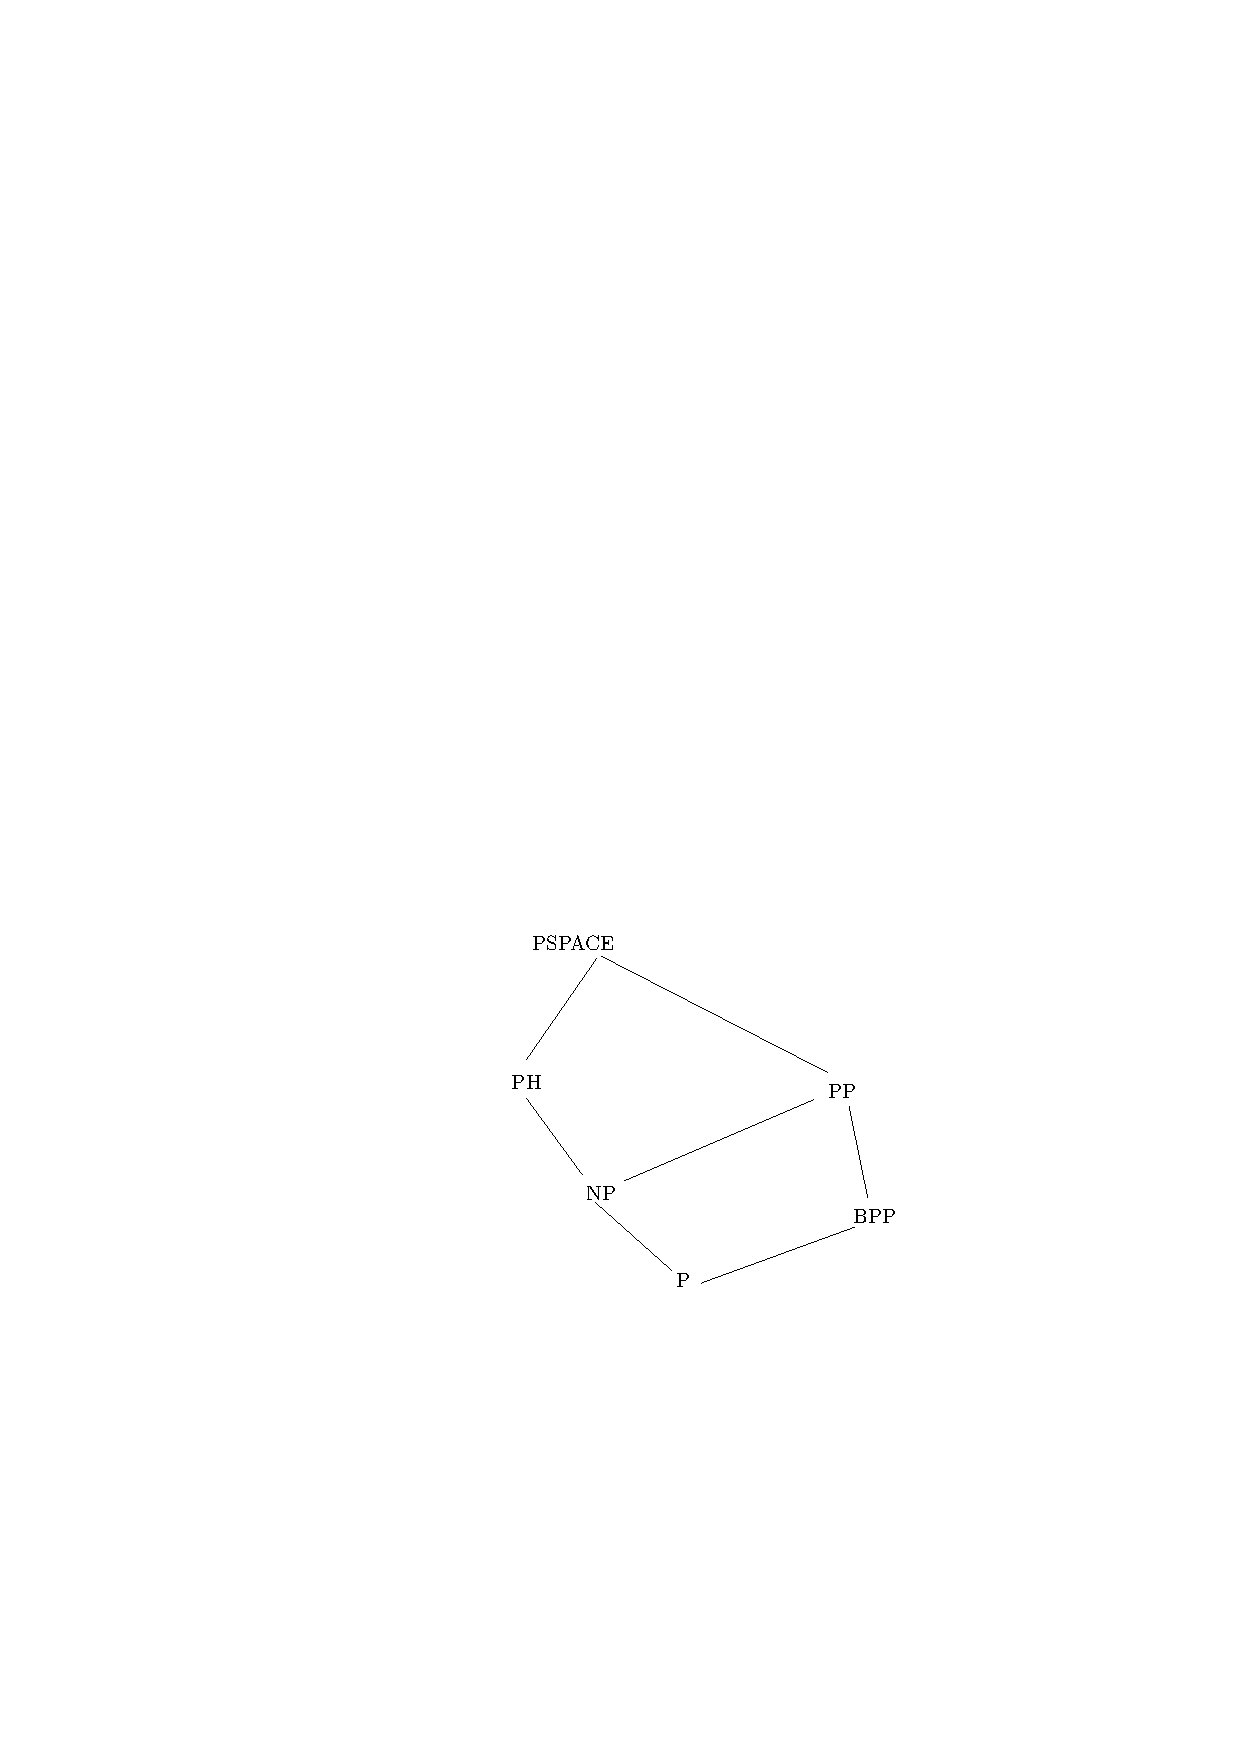
\includegraphics{1.pdf} }
%\end{center}
%\caption{Different Complexity Classes.}
%\label{complexity}
%\end{figure}


\newpage \Lecture{Princy Lunawat}{Jan 25, 2012}{11}{Amplification Lemma}

In the last lecture, we saw the polynomial identity testing problem
and a randomized algorithm for it. We also discussed how branching machines with
guarantees on the number of erroneous paths characterize randomized
algorithms. We ended the last lecture with a question about how two
sets of languages compare. $\BPP_{\epsilon}$ and $\BPP_{\epsilon'}$.
for different $\epsilon$ and $\epsilon'$? 

\section{Amplification of Success Probability}

We showed that if $\epsilon < \epsilon'$ then $\BPP_{\epsilon} \subseteq \BPP_{\epsilon'}$. A strategy to prove the other direction was the following : Repeat the randomized algorithm (experiment) multiple
times (say $k$), and then take the majority of the outcomes in order to improve our success probability.
One remark is that the repetition is sequential and happens on each
branch. Thus we are essentially producing a new branching machine with
many deeper computation paths. 

Why would this improve the success probability? and if so, how does it depend on $k$?. 
The following lemma answers these.

\begin{lemma}
If $\mathcal{E}$ is an event that $Pr(\mathcal{E}) \geq \frac{1}{2} + \epsilon $, then the probability the $\mathcal{E}$ occurs atleast $\frac {k}{2}$ times on $k$ independent trials is at least 
$1-\frac{1}{2}(1-4\epsilon^2)^\frac{k}{2}$
\end{lemma}
\begin{proof}
Let $q$ denote the probability the $\mathcal{E}$ occurs atleast $\frac {k}{2}$ times on $k$ independent trials.
Let $q_i$ = Pr($\mathcal{E}$ occurs exatly $i$ times in $k$ trials), $0 \leq i \leq k$. Thus,
$q = 1 - \sum_{i=0}^{\lfloor\frac{k}{2}\rfloor}$ $q_i$. We will analyse the complementary event:
Pr($\mathcal{E}$ occurs atmost $\frac{k}{2}$ times) = $\sum_{i=0}^{\lfloor\frac{k}{2}\rfloor}$ $q_i$. \\ 
We show an upper bound on each $q_i$ and thus show an lower bound on $q$.
\begin{eqnarray*}
q_i & = & {k \choose i} (\frac{1}{2} + \epsilon)^{i} (\frac{1}{2} - \epsilon)^ {k-i} \\
& \leq & {k\choose i} \left(\frac{1}{2} + \epsilon\right)^{i} \left(\frac{1}{2} - \epsilon\right)^ {k-i} \left(\frac{\frac{1}{2} + \epsilon}{\frac{1}{2} - \epsilon}\right)^{\frac{k}{2} - i}  (because \epsilon \le \frac{1}{2} ) \\
& = & {k\choose i}\left(\frac{1}{2} + \epsilon\right)^{\frac{k}{2}}\left(\frac{1}{2} - \epsilon\right)^{\frac{k}{2}} \\
&= & {k\choose i} \left(\frac{1}{4} - \epsilon^2\right)^{\frac{k}{2}}
\end{eqnarray*}
Now we analyse the sum:
\begin{eqnarray*}
\sum_{i=0}^{\lfloor\frac{k}{2}\rfloor}q_i & \leq & \sum_{i=0}^{\lfloor\frac{k}{2}\rfloor}{k\choose i} \left(\frac{1}{4} - \epsilon^2\right)^{\frac{k}{2}} \\
q = 1 - \sum_{i=0}^{\lfloor\frac{k}{2}\rfloor}q_i & \geq & \sum_{i=0}^{\lfloor\frac{k}{2}\rfloor}{k\choose i} \left(\frac{1}{4} - \epsilon^2\right)^{\frac{k}{2}} \\
& = & 1 - \left(\frac{1}{4} - \epsilon^2\right)^{\frac{k}{2}} 2^{k-1} \\
& = & 1 - \frac{1}{2} \left(1 - 4\epsilon^2\right)^{\frac{k}{2}} \\
\textrm {Thus, } q & \ge & 1 - \frac{1}{2} \left(1 - 4\epsilon^2\right)^{\frac{k}{2}}
\end{eqnarray*}
\end{proof}

In the last lecture, we defined the class $\BPP_\epsilon$ (Bounded Error Probabilistic Polynimial Time) and now we can use the above amplification lemma to prove that
\[\BPP_{\epsilon} = \BPP_{\epsilon^{'}} \hspace{3mm}\forall  0 \leq \epsilon , \epsilon' < \frac{1}{2} \]

We want to calculate
In general, the above lemma can be used to prove that , at the cost of running time, the the error probability of a language $L$ , 
$L \in \BPP$ can be reduced to $\frac{1}{2^{q(n)}}$ where $q(n)$ is a polynomial in $n$.
 
\begin{lemma}
$L \in \BPP$ if an only if for any polynomial $q(n)$ there is a machine $M$ that runs for time $p(n)$ (which depends on $q(n)$) such that \\
\[ \textrm{ Pr($M$ errs on input $x$)) } \le 2^{-q(n)} \] 
In terms of number of paths,
\[ \#err_M(x) \le  2^{p(n)-q(n)} \]
\end{lemma}
\begin{proof}
Given a language $L \in \BPP_\epsilon$ with PTM $M$, we design a PTM $N$ such that $L(N) \in \BPP$ and $L(n) = L$ as follows:
\begin{itemize}
 \item Run the machine $M$ on input $x$ $k$ times independently where choice of $k$ is such that
\\
\begin{equation}\label{eq:eq2}
 \frac{1}{2} \left(1 - 4\epsilon^2\right)^{\frac{k}{2}} \leq 2^{-q(n)}
\end{equation}

\end{itemize}
The above equation $\eqref{eq:eq2}$ yields a value of $k$ polynomial in $n$ and hence $N$ runs a polynomial number of times.
The amplification lemma ensures that the error probability reduces to the LHS of the equation $\eqref{eq:eq2}$.
\end{proof}

\section*{The Structure of \BPP}
We explore some interesting structural properties about the class $\BPP$.

\begin{proposition}
$\BPP$ is closed under complementation.
\end{proposition}
\begin{proof}
Let $L \in BPP$ via PTM $M$ with error probability $\epsilon < \frac{1}{2}$ . We show that $\bar L$ is in $\BPP$.
We design a new machine $\bar M$ by switching the accept and reject states of $M$.
\begin{eqnarray*}
x \in L & \implies & \#acc_M(x) \geq (1 - \epsilon )\#path_M(x) \\
& \implies & \#rej_M(x) \leq \epsilon \#path_M(x). \\
& \implies & \#acc_{\bar M} \leq \epsilon \#path_{\bar M}(x). \\
& \implies & x \notin L(\bar M). \\
x \notin L & \implies & \#acc_M(x) \leq \epsilon.\#path_M(x). \\
& \implies & \#rej_M(x) \geq (1-\epsilon)\#path_M(x). \\
& \implies & \#acc_{\bar M} \geq (1-\epsilon) \#path_{\bar M}(x).\\
& \implies & x \in L(\bar M).
\end{eqnarray*}

Hence, we have,
\[x\in L \iff x\notin L(\bar M) \]
Therefore, $L(\bar M) = \bar L$ and $L \in BPP$ via machine $\bar M$. Hence,
$BPP$ is closed under complementation.
\end{proof}

%\includegraphics[scale=0.5,trim = 10mm 80mm 50mm 5mm]{hie1}
%\pagebreak

\section*{One-sided Error Randomized Algorithms}

Consider the language , PIT that is, Polynomial Identity Testing,
\[PIT =\{ p |  p\equiv 0 \}\] where $p$ is a polynomial.
From, the last lecture, we make the following observation about PIT,
if $p \in PIT$, PTM makes no error,
if $p \notin PIT$, PTM makes some error (less than half the number of paths).

We now explore how complexity theory can be extended to these kind of algorithms too.
\begin{definition}({\bf \RP})
A language $L$ is said to be in $\RP$ if there is an $\epsilon$ such
that $0 < \epsilon < \frac{1}{2}$, and a randomized algorithm $A$ such that :
\begin{eqnarray*}
x \in A & \implies & Pr [\textrm{ $A$ accepts }] \ge \frac{1}{2}+\epsilon \\
x \notin A & \implies & Pr [\textrm{ $A$ accepts }] = 0
\end{eqnarray*}
\end{definition}

Hence we have the following proposition:
\begin{equation}
PIT \in \co\RP
\end{equation}

\begin{proposition}
$\RP \subseteq \NP$
\end{proposition}
\begin{proof}
Consider language $L \in \RP$ via machine $M$ such that 
$x \in L \implies M $ accepts $x$ with some error $\epsilon < \frac{1}{2}$
$\implies M $ accepts $x$ on atleast 1 path. \\
$x \notin L \implies M$ accepts $x$ with probability 0 $\implies M$ rejects on all paths.
Thus $L \in \NP$. Moreover, even with the acceptance condition of a non-deterministic machine, the branching machine corresponding to the $\RP$ algorithm accepts the language $L$ itself.
\end{proof}
\vspace{-40mm}
\begin{center}
\includegraphics[scale=0.3, trim = 30mm 50mm 0mm 5mm, clip]{hie2}
\includegraphics[scale=0.3]{hie3}
\end{center}
\vspace{-10mm}

\section{Derandomization of $\BPP$}
There are several questions connected to the new class $\BPP$ that contains several natural problems. We saw one example of multivariate polynomial identity testing problem. Is $BPP \subseteq P$? This would amount to showing that in the world of efficient computations, randomization does not add any power. There are reasons to remotely believe this to be the case, but till date there is no proof. 

A question of slightly different flavour is, if problems in $\BPP$ are contained in $\NP$? That is, can we trade non-determinism with randomness? We already know that if the randomness causes only one-sided error, then it can be replaced by simple non-deterministm ($\RP \subseteq \NP$). But extending this to two-sided error version is an interesting open problem in the area. 

We show a relaxed containment which can be seen to be an improved upper bound for problems in $\BPP$ compared to the trivial upper bound of $\PSPACE$.

\begin{theorem}
$BPP \in \Sigma_2$
\end{theorem}
\begin{proof}
Let $L \in \BPP$. By using amplification lemma for $q(n) = n$ we can state:
there is a probabilistic Turing machine $M$ and polynomial p(n) such that,
\[\#err_M(x) \leq 2^{-n} 2^{p(n)}\]

Let us recall the definition and a characterization of the class $\Sigma^2$
$\Sigma_2$ is defined as follows:
$L \in \Sigma_2$ iff $\exists B \in P $ such that:
\[x \in L \iff \exists y,  \forall z,  (x,y,z) \in B\]

There is a clear mindblock here. How do we tradeoff quantifiers to randomness?

Let us define a set A(x) as follows:
\[ A(x) = \{y\in \{0,1\}^{p(n)} |  M\ accepts\ x\ on\ path\ y \}\]

Observe that, 
\[x \in L \Rightarrow |A(x)| \geq (1- 2^{-n}) 2^{p(n)} \]
that is, no. of $y$'s such that $M(x,y) = 1$ is large.
\[x \notin L \Rightarrow |A(x)| \leq  2^{-n} 2^{p(n)}) \] 
that is, no, of $y$'s such that $M(x,y) = 1$ is small.
\\

\textbf{Parity Map:}
For two strings $y,z \in \{0,1\}^{p(n)}$, let $y \parity z$ denote the bit-wise parity of the two strings.
We can extend the parity map to operate on subsets of $\{0,1\}^{p(n)}$ as follows:
\[ S \parity z = \{y \parity z ~|~ y \in S \, z \in \{0,1\}^{p(n)} \}\]

\begin{observation}
For a fixed $z$, $\parity_z$ is a bijection from $\{0,1\}^{p(n)} \to \{0,1\}^{p(n)}$. That is, for any $z \in \{0,1\}^{p(n)}$, and $S \subseteq \{0,1\}^{p(n)}$, $|S| =|S \parity z|$.
\end{observation}

Ask the question : how many $z$'s do we need to cover $\{0,1\}^{p(n)}$ entirely?
That is, how large do we need $m$ to be, such that there exists strings $z_1, z_2, \ldots, z_m$ such that:
\[\bigcup_{i=1}^{m} (A(x) \parity z_i) = \{0,1\}^{p(n)}  \]

Intuitively, we expect the answer to be {\em small} when the size of $A(x)$ is large, and {\em large} when the size of $A(x)$ is small. Now we formalize this.

\textbf{Case 1:} Small $|A(x)| \leq 2^{-n} 2^{p(n)}$
In the best case, let each $z_i$ maps $A(x)$ to non-intersecting sets.
\[ \forall i, j (A(x)\parity z_i) \cap (A(x) \parity z_j) = \phi , i \neq j \]
\[|\bigcup_{i=1}^{m} (A(x) \parity z_i)| \geq |\{0,1\}^{p(n)}|\]
\[\Rightarrow m (2^{-n}) 2^{p(n)} \geq 2^{p(n)}\]
\[\Rightarrow m \geq 2^n\]

Hence, the no. of $z$'s required is exponential in $n$ when $A(x)$ is small, that is, when
$x \notin L$.
\\

\textbf{Case 2:} Large $|A(x)| \geq (1 - 2^{-n}) 2^{p(n)}$
We prove that $\exists z_1, z_2, z_3 ... z_m$ for a small $m$ such that 
\[|\bigcup_{i=1}^{m} (A(x) \parity z_i)| = |\{0,1\}^{p(n)}|\]
We call the $m$-tuple $z_1, z_2, z_3 ... z_m$ {\em bad}, if ,
\[|\bigcup_{i=1}^{m} (A(x) \parity z_i)| \neq |\{0,1\}^{p(n)}|\]
\[\Rightarrow \exists w \in \{0,1\}^{p(n)}, z_i \parity y \neq w ,\forall y \in
A(x), \forall i \]
\[\Rightarrow \{z_i \parity w | 1 \leq i \leq m \} \subset R(x)\]
where $R(x) = \bar A(x)$.
$|R(x)| = 2^{p(n)} - |A(x)|$
$\Rightarrow |R(x)| \leq  2^{p(n) - n}$

For a given $w$ and a given subset of $R(x)$ of size $m$, we get a {\em bad} $m$-tuple
$z_1, z_2, z_3 ... z_m$. Hence,
\\
Number of {\em bad} $z_1, z_2, z_3 ... z_m \leq $ Number of of $w$'s $\times$ Number of subsets
of $R(x)$ of size $m$.
\\
$\Rightarrow$ Number of {\em bad} $z_1, z_2, z_3 ... z_m \leq 2^{p(n)} (2 ^{p(n)-n})^m $
\\
Total number of $z_1, z_2, z_3 ... z_m $ = $(2^{p(n)})^m$.
$m$ should be such that,
\[2^{p(n)} (2 ^{p(n)-n})^m < (2^{p(n)})^m\]
\[p(n) + (p(n)-n)m < p(n)m\]
\[p(n) - nm < 0\]
\[m > \frac{p(n)}{n}\]

This goes well with our intuition. If $m$ is allowed to be very small, then we should not be able to cover the entire set $\{0,1\}^n$. For, $m > \frac{p(n)}{n}$ we are guaranteed to have atleast one {\em good} $m$-tuple, that is,
\[z_i \parity w = y , y \in A(x)\]

Hence we conclude that, 
\[\exists z_1, z_2, z_3 ... z_m , \forall w \in \{0,1\}^{p(n)} \left( \bigwedge_{i=1}^{m} \left[~z_i \parity w
\in A(x) ~\right] \right) \]
\[\exists z_1, z_2, z_3 ... z_m , \forall w \in \{0,1\}^{p(n)}, \left( \bigwedge_{i=1}^{m} \left[ ~M(x, z_i
\parity w) = 1 ~\right] \right) \]

Checking if $M$ accepts $x$ on a given path is a polynomial time operation, and
repeating it for each $z_i$ where the number of $z_i$'s is polynomial in $n$ is
also a polynomial time operation. Fix $m = p(n)$, Thus we have a $B \in \P$ such that

\[ x \in L \iff \exists \overline{z} \in \{0,1\}^{p(n)^2}, \forall w \in \{0,1\}^{p(n)} (x,\overline{z},w) \in B \]
Hence, the above language $L \in \Sigma_2$.
\end{proof}
  



\bibliographystyle{abbrv}
\bibliography{references}

\end{document}
